% ---------------------------------------------------------------
% نسخه ی ساده ی گزارش با LaTeX + XePersian
% کامپایل با:  xelatex main.tex   (دو بار، برای فهرست مطالب)
% تنها از یک فونت استفاده می شود: Yas
% ---------------------------------------------------------------
\documentclass[12pt,a4paper]{article}

\usepackage[margin=2.5cm]{geometry}
\usepackage{graphicx}
\usepackage{float}
\usepackage{listings}
\usepackage{tikz}
\usetikzlibrary{positioning}
\usepackage{xepersian}

% ---- فونت: فقط Yas ------------------------------------------
\settextfont{Yas}
\setlatintextfont{Yas}
\setmonofont{Yas}

% ---- تنظیمات کد ----------------------------------------------
\lstset{
  basicstyle=\footnotesize\ttfamily,
  columns=fullflexible,
  keepspaces=true,
  breaklines=true,
  frame=single,
  numbers=none,
  showstringspaces=false,
}

\title{پیاده سازی و تحلیل سیاست های جایگزینی حافظه ی نهان در \lr{ChampSim}}
\author{امیر محمد محقق \and امیررضا دولتی \and سپهر کلانکی \and سینا فعالیت}
\date{تابستان ۱۴۰۴}

\begin{document}

\maketitle
\tableofcontents
\newpage
\section{مقدمه}

مسله ی اصلی که در این پروژه باید بررسی می شد، مطالعه و مقایسه ی \lr{Replacement Policy} های مختلف \lr{Cache} در لایه ی آخر (\lr{LLC}) است. سیاست های بررسی شده در این گزارش به شرح زیرند:

\begin{table}[H]
\centering
\begin{tabular}{|c|c|c|}
\hline
مخفف & نام کامل & مرجع \\
\hline
\lr{LRU} & \lr{Least Recently Used} & ویکی پدیا \cite{wiki_replacement} \\
\hline
\lr{MRU} & \lr{Most Recently Used} & ویکی پدیا \cite{wiki_replacement} \\
\hline
\lr{FIFO} & \lr{First In First Out} & ویکی پدیا \cite{wiki_replacement} \\
\hline
\lr{Random} & \lr{Random Replacement} & ویکی پدیا \cite{wiki_replacement} \\
\hline
\lr{SRRIP} & \lr{Static Re-Reference Interval Prediction} & مقاله ی \lr{RRIP} \cite{jaleel2010rrip} \\
\hline
\lr{DRRIP} & \lr{Dynamic Re-Reference Interval Prediction} & مقاله ی \lr{RRIP} \cite{jaleel2010rrip} \\
\hline
\lr{BIP} & \lr{Bimodal Insertion Policy} & مقاله ی \lr{DIP} \cite{qureshi2007dip} \\
\hline
\lr{SHiP} & \lr{Signature-based Hit Predictor} & مقاله ی \lr{SHiP} \cite{wu2011ship} \\
\hline
\end{tabular}
\caption{سیاست های جایگزینی بررسی شده در این پروژه}
\end{table}

شبیه سازی ها همگی با شبیه ساز \lr{ChampSim} \cite{gober2022champsim} انجام شده اند و ردپا های استفاده شده را از مخزن ردپا های آماده ی \lr{ChampSim} دانلود کرده ایم \cite{champsim_traces}.

\begin{quote}
برای بخش امتیازی ما تغییر تعداد \lr{set} ها را انتخاب کردیم و بین مقادیر ۱۰۲۴ و ۲۰۴۸ و ۴۰۹۶ تغییرشان دادیم. تحلیل های خارج از حالت امتیازی روی ۲۰۴۸ انجام شده اند.
\end{quote}

\begin{quote}
تعداد دستورات برای بخش \lr{warmup} برابر ۱۲٫۵ میلیون و برای بخش شبیه سازی برابر ۵۰ میلیون است.
\end{quote}

\newpage
\section{توضیح \lr{Replacement Policy} ها}

برای تمام \lr{Replacement Policy} ها یک دور روش آنها را به طور کامل توضیح می دهیم که گزارش کامل باشد.
نکات ناقص رو نیز باید اضافه بکنیم.

\subsection{یک نکته ی مشترک بین چند \lr{policy}: نوع دسترسی \lr{access\_type::WRITE}}

در چند تا از سیاست های، یک شرط روی \lr{\texttt{access\_type}} می بینیم که دسترسی های نوع \lr{WRITE} را جدا می کند. این نوع دسترسی ها مربوط به \lr{writeback} می شود. نکته این است که این نوشتن نشانه ی استفاده ی پردازنده از داده در همان لحظه نیست، بلکه صرفا نتیجه ی \lr{replacement} در سطح بالاتر است. اگر \lr{writeback} ها را مثل دسترسی عادی حساب کنیم و سیاست ها را روی آنها نیز اجرا کنیم، دو مشکل پیش می آید: اول اینکه بلوک هایی که فقط نوشته شده اند بی دلیل تازه به حساب می آیند و در کش ماندگار می شوند و دوم اینکه در سیاست های پویا مثل \lr{DRRIP} آمار تصمیم گیری منحرف می شود چون این دسترسی ها رفتار واقعی برنامه را نشان نمی دهند. به همین دلیل در سیاست های ما یا اثر \lr{writeback} نادیده گرفته می شود یا بلوک با یک مقدار امن و غیر مخرب پر می شود.

\subsection{توابع مهم برای هر سیاست}

\begin{itemize}
  \item تابع \lr{\texttt{find\_victim}}: وقتی \lr{miss} رخ داد، شماره ی \lr{way} قربانی را برمی گرداند.
  \item تابع \lr{\texttt{replacement\_cache\_fill}}: بعد از اینکه بلوک جدید داخل \lr{way} قرار گرفت صدا زده می شود (منطق \lr{fill}).
  \item تابع \lr{\texttt{update\_replacement\_state}}: در هر دسترسی صدا زده می شود و پارامتر \lr{\texttt{hit}} مشخص می کند دسترسی \lr{hit} بوده یا نه.
\end{itemize}

نکته ی نهایی این نیز که بیشتر تنظیمات کلی و \lr{global} به ازای هر \lr{CPU Core} است، مثلا برای شمارنده ها و ...

\subsection{\lr{LRU}}

منطق انتخاب بلوک قربانی:

بین تمام بلوک های موجود در یک \lr{set}، بلوکی حذف می شود که بیشترین زمان بدون استفاده مانده است، به همین دلیل بلوک های که دسترسی بیشتری در طول زمان دارند کمتر حذف می شوند.

نحوه بروزرسانی اطلاعات کمکی:

هر بلوک یک مقدار زمان دسترسی نگه می دارد که نشان می دهد نسبت به بقیه بلوک ها داخل همان \lr{set} کی مورد دسترسی واقع شده است. مقدار ۰ یعنی اینکه نسبت به بقیه قدیمی تر استفاده شده است، و هرچه مقدار آن بزرگتر باشد یعنی اینکه نسبت به بقیه جدید تر مورد دسترسی واقع شده است، و جدیدترین دسترسی این \lr{set} است. هر دسترسی با توجه به \lr{Miss} یا \lr{Hit} شدن مقادیر را تغییر می دهیم که ترتیب دسترسی حفظ شود.

نحوه ی بروزرسانی اطلاعات پس از برخورد (\lr{hit}):

در هنگام \lr{hit} برچسب زمان همان بلوک برابر مقدار فعلی شمارنده ی \lr{\texttt{cycle}} می شود و بعد \lr{\texttt{cycle}} یکی زیاد می شود. یعنی آن بلوک تبدیل به جدیدترین بلوک (\lr{MRU}) در \lr{set} خودش می شود و برچسب بقیه ی بلوک ها دست نخورده باقی می ماند، پس به صورت نسبی همه ی آنها یک واحد زمانی قدیمی تر می شوند. تنها استثنا دسترسی های نوع \lr{WRITE} است که مطابق توضیح ابتدای بخش نادیده گرفته می شوند و برچسب زمان را عوض نمی کنند.

نحوه ی بروزرسانی اطلاعات پس از جایگزینی (\lr{fill}):

بعد از اینکه بلوک قربانی خارج شد و بلوک جدید در همان \lr{way} نشست، تابع \lr{\texttt{replacement\_cache\_fill}} برچسب زمان آن \lr{way} را برابر \lr{\texttt{cycle}} قرار می دهد و شمارنده را زیاد می کند. پس بلوک تازه درج شده در موقعیت \lr{MRU} قرار می گیرد و امن ترین بلوک \lr{set} است، یعنی تا وقتی که تمام بلوک های دیگر یک بار خارج نشوند نوبت به آن نمی رسد. هیچ اطلاعات دیگری در \lr{set} بروزرسانی نمی شود.

شرایط عملکرد مناسب و نامناسب:

سیاست \lr{LRU} وقتی خوب کار می کند که برنامه از داده هایی که استفاده می کند به تعداد بالاتری نیز مجدد استفاده بکند.

در مقابل، \lr{LRU} در حالت های \lr{scan} های خطی یا حلقه ای که در \lr{cache} جا نشوند بد عمل می کند، چون به ترتیب داده ها یکبار مصرف می شوند و در دومی تا به سر آرایه برسیم آن داده ها دور ریخته شده اند و عملا فقط \lr{cache} را کثیف کردیم.

نکات کد:

\subsubsection{قطعه ۱ — ساختار داده ی کمکی و سازنده}

\begin{latin}
\begin{lstlisting}
class lru : public champsim::modules::replacement
{
  long NUM_WAY;
  std::vector<uint64_t> last_used_cycles;
  uint64_t cycle = 0;
  ...
};

lru::lru(CACHE* cache) : lru(cache, cache->NUM_SET, cache->NUM_WAY) {}

lru::lru(CACHE* cache, long sets, long ways)
    : replacement(cache), NUM_WAY(ways),
      last_used_cycles(static_cast<std::size_t>(sets * ways), 0) {}
\end{lstlisting}
\end{latin}

اطلاعات اضافه در یک بردار یک-بعدی به طول \lr{\texttt{sets * ways}} نگه داری می شود و آدرس هر بلوک با فرمول \lr{\texttt{set * NUM\_WAY + way}} به دست می آید.

\subsubsection{قطعه ۲ — انتخاب بلوک قربانی}

\begin{latin}
\begin{lstlisting}
long lru::find_victim(uint32_t triggering_cpu, uint64_t instr_id, long set, ...)
{
  auto begin = std::next(std::begin(last_used_cycles), set * NUM_WAY);
  auto end = std::next(begin, NUM_WAY);

  // Find the way whose last use cycle is most distant
  auto victim = std::min_element(begin, end);
  assert(begin <= victim);
  assert(victim < end);
  return std::distance(begin, victim);
}
\end{lstlisting}
\end{latin}

ابتدا با \lr{\texttt{begin}} و \lr{\texttt{end}} بازه ی مربوط به همان \lr{set} جدا می شود و بعد \lr{\texttt{min\_element}} کوچک ترین برچسب زمان را پیدا می کند. چون برچسب بزرگ تر یعنی دسترسی جدیدتر، کوچک ترین مقدار دقیقا یعنی بلوکی که از همه دیرتر استفاده شده است.

اگر چند بلوک مقدار برابر داشته باشند (مثلا چند \lr{way} هنوز دست نخورده و برابر ۰ باشند)، \lr{\texttt{min\_element}} اولین آنها را برمی گرداند، پس ترتیب پر شدن \lr{set} از \lr{way} کوچک به بزرگ است.

\subsubsection{قطعه ۳ — درج و به روزرسانی}

\begin{latin}
\begin{lstlisting}
void lru::replacement_cache_fill(uint32_t triggering_cpu, long set, long way, ...)
{
  // Mark the way as being used on the current cycle
  last_used_cycles.at((std::size_t)(set * NUM_WAY + way)) = cycle++;
}

void lru::update_replacement_state(..., uint8_t hit)
{
  // Mark the way as being used on the current cycle
  if (hit && access_type{type} != access_type::WRITE) // Skip this for writeback hits
    last_used_cycles.at((std::size_t)(set * NUM_WAY + way)) = cycle++;
}
\end{lstlisting}
\end{latin}

در زمان درج بلوک جدید در موقعیت \lr{MRU} قرار می گیرد و کم خطر ترین بلوک \lr{set} است.

\subsection{\lr{FIFO}}

منطق انتخاب بلوک قربانی:

بین تمام بلوک های موجود در \lr{set}، بلوکی که زودتر از همه وارد شده است باید خارج شود (منطق \lr{First In First Out}). اینکه بلوک اخیرا دسترسی قرار گرفته یا نه تاثیری در تصمیم گیری ندارد. عملا منطق صف دارد.

نحوه بروزرسانی اطلاعات کمکی:

یک ترتیب ورود برای بلوک هایی که به \lr{set} وارد می شوند ذخیره می کند. موقع \lr{hit} چیزی را تغییر نمی دهد ولی موقع \lr{miss} ترتیب عوض می شود (البته بدون آپدیت کردن مقدار بقیه چون زمان اضافه شدن اهمیت دارد).

نحوه ی بروزرسانی اطلاعات پس از برخورد (\lr{hit}):

هیچ بروزرسانی ای انجام نمی شود و تابع \lr{\texttt{update\_replacement\_state}} کاملا خالی است.

نحوه ی بروزرسانی اطلاعات پس از جایگزینی (\lr{fill}):

بعد از درج بلوک جدید، برچسب آن \lr{way} برابر مقدار فعلی \lr{\texttt{cycle}} قرار می گیرد و شمارنده یکی زیاد می شود، یعنی بلوک جدید به انتهای صف اضافه می شود. برچسب بقیه ی بلوک ها دست نمی خورد چون ترتیب ورود آنها ثابت است و ربطی به بلوک جدید ندارد.

شرایط عملکرد مناسب و نامناسب:

سیاست \lr{FIFO} وقتی خوب عمل می کند که ترتیب ورودی داده ها با ترتیب استفاده از آنها هماهنگ باشد.

در جاهایی بد عمل می کند که بلوکی زود وارد \lr{cache} شود ولی چون صرفا زود وارد شده ممکن است با اینکه در آینده ی نزدیک خیلی استفاده می شود دور ریخته شود، و هوشمندی این را ندارد که اگر یک بلوک زیاد استفاده می شود نباید سریع بیرون بیندازدش.

نکات کد:

\subsubsection{قطعه ۱ — ساختار داده}

\begin{latin}
\begin{lstlisting}
class fifo : public champsim::modules::replacement
{
  long NUM_WAY;
  std::vector<uint64_t> insertion_cycles;
  uint64_t cycle = 0;
  ...
};
\end{lstlisting}
\end{latin}

ساختار داده دقیقا مثل \lr{LRU} است و تنها چیزی که فرق می کند مفهوم عدد کمکی است، که اینجا مفهوم زمان وارد شدن بلوک به \lr{set} را می دهد. \lr{\texttt{cycle}} در اینجا یک شمارنده کلی است که برای زمان اضافه شدن استفاده می شود و بیانگر شمارشگر زمان است که در هنگام هر \lr{fill} افزایش پیدا می کند.

\subsubsection{قطعه ۲ — انتخاب قربانی و ثبت زمان ورود}

\begin{latin}
\begin{lstlisting}
long fifo::find_victim(uint32_t triggering_cpu, uint64_t instr_id, long set, ...)
{
    auto begin = std::next(std::begin(insertion_cycles), set * NUM_WAY);
    auto end = std::next(begin, NUM_WAY);

    // Evict the oldest inserted block
    auto victim = std::min_element(begin, end);
    return std::distance(begin, victim);
}

void fifo::replacement_cache_fill(uint32_t triggering_cpu, long set, long way, ...)
{
    // Record insertion time
    insertion_cycles.at((std::size_t)(set * NUM_WAY + way)) = cycle++;
}
\end{lstlisting}
\end{latin}

بدون اینکه صف واقعی داشته باشیم، با یک برچسب زمان ورود همان رفتار صف را می سازیم، کمترین مقدار یعنی قدیمی ترین ورود که همان بلوک از صف خارج می شود.

\subsubsection{قطعه ۳ — تابع خالی به روزرسانی}

\begin{latin}
\begin{lstlisting}
void fifo::update_replacement_state(..., uint8_t hit)
{
}
\end{lstlisting}
\end{latin}

تابع \lr{update} این \lr{policy} خالی است چون طبق توضیحات در \lr{FIFO} لازم نیست کاری انجام بدهیم.

\subsection{\lr{MRU}}

منطق انتخاب بلوک قربانی:

کاملا مخالف \lr{LRU} عمل می کند ولی منطق مشابهی دارد به این صورت که بلوکی در \lr{set} خارج می شود که نسبت به بقیه اخیرا دسترسی داشته است.

نحوه بروزرسانی اطلاعات کمکی:

مشابه \lr{LRU} و نکته ای اضافه ای ندارد.

نحوه ی بروزرسانی اطلاعات پس از برخورد (\lr{hit}):

دقیقا مثل \lr{LRU}، برچسب زمان بلوکی که \lr{hit} شده برابر \lr{\texttt{cycle}} می شود و شمارنده زیاد می شود (و باز هم دسترسی های \lr{WRITE} نادیده گرفته می شوند). ولی معنای این کار برعکس \lr{LRU} است.

نحوه ی بروزرسانی اطلاعات پس از جایگزینی (\lr{fill}):

بلوک تازه \lr{fill} شده بزرگترین برچسب زمان \lr{set} را می گیرد، پس بلافاصله پرخطرترین بلوک برای خروج می شود.

شرایط عملکرد مناسب و نامناسب:

می شود گفت نقطه ی مقابل \lr{LRU} است و هر جا آن بد عمل می کند این خوب عمل می کند و هر جا آن خوب عمل می کند این بد عمل می کند. صرفا اینکه برای ذخیره ی استفاده ی مکرر از داده های جدید خیلی بد عمل می کند.

نکات کد:

\subsubsection{قطعه ۱ — تنها تفاوت با \lr{LRU}}

\begin{latin}
\begin{lstlisting}
long mru::find_victim(uint32_t triggering_cpu, uint64_t instr_id, long set, ...)
{
  auto begin = std::next(std::begin(last_used_cycles), set * NUM_WAY);
  auto end = std::next(begin, NUM_WAY);

  auto victim = std::max_element(begin, end); //MRU!!!
  return std::distance(begin, victim);
}
\end{lstlisting}
\end{latin}

کل تفاوت پیاده سازی با \lr{LRU} استفاده از \lr{\texttt{max\_element}} به جای \lr{\texttt{min\_element}} است، به همین دلیل بلوکی که اخیرا به \lr{set} اضافه شده است قربانی است. بقیه ی کد ها با \lr{LRU} کاملا یکسان هستند.

\subsection{\lr{Random}}

منطق انتخاب بلوک قربانی:

در هر \lr{set} به صورت رندوم یک بلوک را انتخاب می کنیم.

نحوه بروزرسانی اطلاعات کمکی:

اطلاعات اضافه ای برای ذخیره لازم نداریم.

نحوه ی بروزرسانی اطلاعات پس از برخورد (\lr{hit}):

هیچ چیزی بروزرسانی نمی شود و اصلا تابع \lr{\texttt{update\_replacement\_state}} را \lr{override} نکرده ایم، چون هیچ حالتی برای نگه داشتن وجود ندارد. تنها چیزی که با هر انتخاب قربانی تغییر می کند وضعیت داخلی \lr{generator} شبه تصادفی است.

نحوه ی بروزرسانی اطلاعات پس از جایگزینی (\lr{fill}):

اینجا هم هیچ کاری انجام نمی شود و \lr{\texttt{replacement\_cache\_fill}} خالی است.

شرایط عملکرد مناسب و نامناسب:

سیاست \lr{Random} وقتی نسبتا خوب عمل می کند که پترن دسترسی برنامه بدون منطق مشخص و رندوم باشد. صرفا یک روش نامنظم در برابر نامنظم است که لزوما بهترین نتیجه را نمی دهد و یک روش ساده ی نسبتا معمولی است.

در برنامه هایی که پترن مشخص مثل \lr{scan} خطی و استفاده ی مکرر از داده ها دارند اصلا خوب عمل نمی کند چون یک رفتار نامنظم در برابر یک رفتار منظم است.

نکات کد:

\subsubsection{قطعه ۱ — مولد شبه تصادفی و بازه ی انتخاب}

\begin{latin}
\begin{lstlisting}
struct random : public champsim::modules::replacement {
  std::mt19937_64 rng{};
  std::uniform_int_distribution<long> dist;
  ...
};

random::random(CACHE* cache) : random(cache, cache->NUM_WAY) {}

random::random(CACHE* cache, long ways) : replacement(cache), dist(0, ways - 1) {}
\end{lstlisting}
\end{latin}

رندوم روی بازه ی \lr{\texttt{[0, ways-1]}} یک عدد انتخاب می کنیم که بیانگر آن بلوکی است که باید حذف شود.

\subsubsection{قطعه ۲ — انتخاب قربانی و نبود توابع دیگر}

\begin{latin}
\begin{lstlisting}
long random::find_victim(uint32_t triggering_cpu, uint64_t instr_id, long set, ...)
{
  return dist(rng);
}
\end{lstlisting}
\end{latin}

در سیاست \lr{random} کل خطی که منطق این سیاست را پیاده سازی می کند همین است و توابع دیگر نیاز به \lr{override} کردن ندارند چون این سیاست منطق هندل کردن حالت ندارد.

\subsection{\lr{SRRIP}}

به ازای هر بلوک در \lr{set} یک عدد به نام \lr{RRPV} (\lr{Re-Reference Prediction Value}) ذخیره می شود که معمولا ۲ بیت است که ۴ مقدار می تواند به خود بگیرد. در صورتی که ۰ باشد یعنی اینکه احتمالا به زودی استفاده می شود و در صورتی که ۳ باشد احتمالا خیلی در آینده ی دور استفاده می شود و در آینده ی نزدیک احتمالا استفاده نمی شود.

منطق انتخاب بلوک قربانی:

در روش \lr{SRRIP} (\lr{Static Re-Reference Interval Prediction}) کل منطق بر این است که در یک \lr{set} بلوک هایی که خیلی استفاده می شوند پایدار می شوند و در صورتی که استفاده ی یک بلوک کم شود احتمالا بلوک قربانی خواهد بود. برای پیدا کردن بلوک قربانی هم بلوکی که \lr{RRPV} برابر ۳ (بیشترین مقدار) را دارد خارج می شود. و در صورتی که هیچ بلوکی مقدار ۳ نداشت، مقدار \lr{RRPV} تمام بلوک ها را زیاد می کنیم تا یکی به ۳ برسد، و این فرایند تا شرط برقرار شود ادامه پیدا می کند. (بخشی از بروزرسانی هم انجام می دهد)

نحوه بروزرسانی اطلاعات کمکی:

در صورتی که بلوک جدید اضافه شود، یک بلوک با \lr{RRPV} تقریبا میانه مثل \lr{\texttt{MAX\_RRPV-1}} اضافه می کند. در هنگام \lr{hit} مقدار \lr{RRPV} آن بلوک به ۰ ریست می شود. مقدار بروزرسانی هنگام خارج شدن یک بلوک هم داریم که بالا توضیح دادیم.

نحوه ی بروزرسانی اطلاعات پس از برخورد (\lr{hit}):

مقدار \lr{RRPV} بلوکی که \lr{hit} شده به ۰ ریست می شود، یعنی پیش بینی می کنیم که خیلی زود دوباره استفاده می شود و آن را به امن ترین حالت می بریم.

نحوه ی بروزرسانی اطلاعات پس از جایگزینی (\lr{fill}):

ابتدا در خود \lr{\texttt{find\_victim}} و قبل از \lr{fill} کردن، اگر بیشترین \lr{RRPV} موجود در \lr{set} کمتر از \lr{\texttt{maxRRPV}} باشد به همه ی بلوک های آن \lr{set} به اندازه ی \lr{\texttt{diff = maxRRPV - max}} اضافه می شود تا قربانی مشخص شود. بعد از آن برای بلوک تازه اضافه شده مقدار \lr{\texttt{maxRRPV - 1}} می دهیم.

شرایط عملکرد مناسب و نامناسب:

صرفا یک \lr{LRU} پیشرفته تر است، پس یکم هوشمندانه تر از \lr{LRU} عمل می کند و حالت های خوب آن مثل \lr{scan} های خطی و ... است. که چون کمی هوشمندانه تر عمل می کند از \lr{LRU} هم بهتر عمل می کند.

حالت های بد آن تقریبا مشابه \lr{LRU} وقتی است که در اسکن حلقه ای \lr{cache} پر شود و قبل از اینکه به سر حلقه برسیم داده های اولیه دور ریخته شوند و مجدد از اول باید دریافت شوند که همه چیز هدر می رود.

نکات کد:

\subsubsection{قطعه ۱ — \lr{helper} هر \lr{set} و مقداردهی اولیه}

\begin{latin}
\begin{lstlisting}
struct srrip_set_helper {
  using rrpv_type = int;
  static constexpr rrpv_type maxRRPV = 3;

  std::vector<rrpv_type> rrpv_values;
  rrpv_type& get_rrpv(long way);

  long victim();
  void update(long way, bool hit);
};

srrip_set_helper::srrip_set_helper(long ways)
    : rrpv_values(static_cast<std::size_t>(ways), maxRRPV) {}

srrip::srrip(CACHE* cache, long sets_, long ways_) : replacement(cache)
{
  std::generate_n(std::back_inserter(sets), sets_,
                  [ways = ways_] { return srrip_set_helper{ways}; });
}
\end{lstlisting}
\end{latin}

برای داده های کمکی یک شی \lr{\texttt{srrip\_set\_helper}} تعریف می کنیم که داده های مورد نیاز را به صورت گروهی نگه دارد.

مقدار اولیه ی همه ی \lr{way} ها \lr{\texttt{maxRRPV}} است، یعنی کش خالی طوری رفتار می کند که انگار همه ی بلوک ها در مرز خروج هستند. با این حرکت \lr{way} های خالی بدون هیچ بررسی اضافه ای اول از همه انتخاب می شوند.

در اینجا ما \lr{\texttt{maxRRPV}} را مساوی ۳ قرار دادیم که بیانگر همان ۲ بیت برای این داده است.

\subsubsection{قطعه ۲ — انتخاب قربانی و افزایش گروهی}

\begin{latin}
\begin{lstlisting}
long srrip_set_helper::victim()
{
  // Find the maximum RRPV
  auto victim = std::max_element(std::begin(rrpv_values), std::end(rrpv_values));

  // If the maximum element has RRPV less than the maximum, increment everything to the maximum
  std::transform(std::cbegin(rrpv_values), std::cend(rrpv_values), std::begin(rrpv_values),
                 [diff = maxRRPV - *victim](auto x) { return x + diff; });

  // Return the way index
  return std::distance(std::begin(rrpv_values), victim);
}
\end{lstlisting}
\end{latin}

همان توصیف حلقه شکلی که در توضیح سیاست داشتیم اینجا به صورت یک عبارت جبری ساده به صورت \lr{\texttt{diff = maxRRPV - max}} است که به همه اضافه می شود. عملا همان کار حلقه را می کند و این دو روش هم ارزند ولی این بار محاسباتی کمتری دارد.

اگر از قبل بلوکی با مقدار بیشینه وجود داشته باشد، \lr{\texttt{diff}} برابر صفر می شود و \lr{\texttt{transform}} عملا هیچ تغییری نمی دهد. یعنی همان حالت عادی که مستقیما قربانی پیدا می شود.

نکته ی دیگر این است که این افزایش فقط در مسیر \lr{miss} اتفاق می افتد.

\subsubsection{قطعه ۳ — به روزرسانی مشترک برای \lr{hit} و \lr{fill}}

\begin{latin}
\begin{lstlisting}
void srrip_set_helper::update(long way, bool hit) { get_rrpv(way) = hit ? 0 : (maxRRPV - 1); }

void srrip::update_replacement_state(..., uint8_t hit)
{
  sets.at(static_cast<std::size_t>(set)).update(way, hit);
}
\end{lstlisting}
\end{latin}

کد \lr{\texttt{replacement\_cache\_fill}} بازنویسی نشده است و هر دو حالت \lr{hit} و \lr{fill} از همین یک تابع استفاده می کنند که برای اینکه بین \lr{hit} و \lr{fill} تشخیص دهیم یک \lr{\texttt{bool hit}} داریم که بین این دو انتخاب کند.

در صورتی که \lr{hit} بشود مقدار به ۰ ریست می شود و در صورتی که \lr{fill} باشد مقدار جدید برابر \lr{\texttt{maxRRPV-1}} خواهد بود.

\subsection{\lr{BIP}}

منطق انتخاب بلوک قربانی:

روش \lr{BIP} (\lr{Bimodal Insertion Policy}) عملا روی روش \lr{LRU} سوار شده است که منطق خارج کردن بلوک از \lr{set} آن دقیقا مشابه \lr{LRU} است. صرفا نحوه ی هندل کردن ترتیب بلوک ها بر اساس دسترسی اخیر آنها کمی متفاوت است.

نحوه بروزرسانی اطلاعات کمکی:

در روش \lr{LRU} در هنگامی که بلوک جدید اضافه می شود، نسبت به بقیه در ترتیب دسترسی بالاتر بود. ولی در این روش هنگامی که بلوک جدید اضافه می شود با یک احتمال مشخص زیادی در ترتیب دسترسی پایینترین خواهد بود (\lr{Least Recently Used}) که یعنی در خطر خارج شدن است (بر خلاف روش عادی که بلوکی که جدید اضافه می شد کم خطر ترین برای خارج شدن بود) و با یک احتمال متمم مشخص دیگری در ترتیب دسترسی نسبت به بقیه بالاترین خواهد بود (مثل حالت عادی روش \lr{LRU}).

نحوه ی بروزرسانی اطلاعات پس از برخورد (\lr{hit}):

در هنگام \lr{hit} دقیقا مثل \lr{LRU} عمل می کنیم و برچسب زمان بلوک برابر \lr{\texttt{cycle}} می شود و شمارنده زیاد می شود (باز هم به جز دسترسی های \lr{WRITE}).

نحوه ی بروزرسانی اطلاعات پس از جایگزینی (\lr{fill}):

بعد از \lr{fill} کردن، با احتمال ۱/۳۲ برچسب زمان برابر \lr{\texttt{cycle}} می شود (درج در موقعیت \lr{MRU}، مثل \lr{LRU}) و با احتمال ۳۱/۳۲ برچسب برابر ۰ قرار می گیرد که یعنی درج در موقعیت \lr{LRU}. پس به احتمال زیاد بلوک جدید در اولین \lr{miss} بعدی همان \lr{set} دوباره خارج می شود و محتوای قدیمی \lr{set} تقریبا دست نخورده باقی می ماند. آن احتمال کوچک ۱/۳۲ هم برای این است که اگر \lr{working set} برنامه عوض شد، کش بتواند به تدریج محتوای جدید را بپذیرد و برای همیشه روی داده های قدیمی قفل نشود.

شرایط عملکرد مناسب و نامناسب:

در این روش هم مشکل \lr{scan} های حلقه ای که از سایز \lr{cache} بزرگ تر می شوند تا حدی رفع می شود و هم اسکن های خطی که داده های بدردنخور اضافه می شود و فقط یکبار استفاده می شوند، چون یک روش میانی بین \lr{LRU} و \lr{MRU} است این امکان به وجود می آید. چون با یک احتمال کم بعضی داده ها را نگه می دارد و خیلی ها را دور می اندازد، باعث نمی شود که همه چیز یادمان برود و خیلی چیز ها نگه داشته می شوند؛ در اسکن های خطی هم داده های یکبار مصرف اکثرا دور ریخته می شوند و فقط بخش کمی از آنها نگه داشته می شود.

در جایی بد عمل می کند که کل \lr{working set} داخل \lr{cache} جا شود و صرفا بخاطر بدبینی این سیاست خیلی از داده ها بیرون ریخته شوند.

نکات کد:

\subsubsection{قطعه ۱ — مولد تصادفی و پارامتر $\varepsilon$}

\begin{latin}
\begin{lstlisting}
class bip : public champsim::modules::replacement
{
    long NUM_WAY;
    std::vector<uint64_t> last_used_cycles;
    uint64_t cycle = 0;
    std::mt19937 rng;
    std::uniform_int_distribution<int> dist;
    ...
};

bip::bip(CACHE* cache, long sets, long ways)
    : replacement(cache),
      NUM_WAY(ways),
      last_used_cycles((std::size_t)(sets * ways), 0),
      rng(0),
      dist(0, 31)        // 1/32 probability
{
}
\end{lstlisting}
\end{latin}

طبق توزیع \lr{\texttt{dist(0, 31)}} و شرطی که در قطعه ی سوم می آید (\lr{\texttt{== 0}}) یعنی احتمال درج در موقعیت \lr{MRU} دقیقا ۱/۳۲ و احتمال درج در موقعیت \lr{LRU} برابر ۳۱/۳۲ است. (این همان احتمال هایی است که در توضیح این \lr{policy} شرح دادیم) این مقدار به صورت رسمی $\varepsilon$ نام دارد و انتخاب آن دلخواه نیست و باید هوشمندانه باشد، ولی مقدار معمولی آن همین است. باید آنقدر کوچک باشد که برای جست و جوی خطی حافظه باعث \lr{cache pollution} نشود (داده های الکی و اضافه پر نکند) و آنقدر بزرگ باشد که اگر \lr{working set} برنامه عوض شد، \lr{cache} بتواند محتوای جدید را کم کم بپذیرد.

برای \lr{seed} برای رندوم هم \lr{\texttt{rng(0)}} صفر را می دهیم.

بقیه ی ساختار داده دقیقا همان \lr{LRU} است.

\subsubsection{قطعه ۲ — انتخاب قربانی (کاملا مثل \lr{LRU})}

\begin{latin}
\begin{lstlisting}
long bip::find_victim(uint32_t, uint64_t, long set, ...)
{
    auto begin = std::next(last_used_cycles.begin(), set * NUM_WAY);
    auto end = std::next(begin, NUM_WAY);

    auto victim = std::min_element(begin, end);
    return std::distance(begin, victim);
}
\end{lstlisting}
\end{latin}

کاملا مشابه \lr{LRU} برای قربانی عمل می کنیم و منطق پیشرفته تری ندارد.

\subsubsection{قطعه ۳ — درج دو حالته}

\begin{latin}
\begin{lstlisting}
void bip::replacement_cache_fill(uint32_t, long set, long way, ...)
{
    auto idx = (std::size_t)(set * NUM_WAY + way);

    // 1/32 insert at MRU
    if (dist(rng) == 0)
    {
        last_used_cycles[idx] = cycle++;
    }
    else
    {
        // Insert as LRU
        last_used_cycles[idx] = 0;
    }
}

void bip::update_replacement_state(..., uint8_t hit)
{
    if (hit && type != access_type::WRITE)
    {
        last_used_cycles[(std::size_t)(set * NUM_WAY + way)] = cycle++;
    }
}
\end{lstlisting}
\end{latin}

فقط منطق \lr{fill} طبق توضیحی که دادیم فرق می کرد و بقیه کاملا مشابهند.

\subsection{\lr{DRRIP}}

منطق انتخاب بلوک قربانی:

در روش \lr{DRRIP} (\lr{Dynamic RRIP}) منطق خارج کردن بلوک دقیقا مشابه روش \lr{SRRIP} است و تفاوتی ندارد.

نحوه بروزرسانی اطلاعات کمکی:

این روش هم چون یک روش تکمیلی روی \lr{SRRIP} است تقریبا مشابه عمل می کند به جز قراردادی که در هنگام اضافه کردن بلوک به \lr{set} دارد. به این صورت عمل می کند که دو تا \lr{sub-policy} دارد که بین این دوتا به صورت پویا عوض می کند. \lr{sub-policy} اول به این صورت است که برای بلوک جدیدی که اضافه می شود مثل \lr{SRRIP} برای مقدار \lr{RRPV} آن \lr{\texttt{MAX\_RRPV-1}} را قرار دهیم. و \lr{sub-policy} دیگر این است که مثل \lr{BIP}، با احتمال خیلی زیاد (ممکن است پیاده سازی این مورد به صورت احتمالی نباشد، مثلا در پیاده سازی ما اینطور نیست) مقدار \lr{RRPV} آن را \lr{\texttt{MAX\_RRPV}} قرار دهیم (مرز خروجی)، و با احتمال خیلی کمتر \lr{\texttt{MAX\_RRPV-1}} را قرار دهیم. در این روش اینکه کدام یک از این \lr{sub-policy} ها انتخاب می شود با استفاده از روش \lr{set-dueling} انجام می شود. به این صورت که ما ۳ نوع دسته داریم: \lr{brrip\_leader} و \lr{srrip\_leader} و \lr{follower}. برای دسته های \lr{srrip\_leader} و \lr{brrip\_leader} به صورت ثابت به ترتیب از \lr{sub-policy} های \lr{SRRIP} و \lr{BRRIP} استفاده می کنیم ولی برای دسته آخر که \lr{follower} است با توجه به یک شمارنده \lr{PSEL} انجام می شود.

هنگام \lr{hit} هم فارغ از اینکه \lr{sub-policy} کدام باشد مقدار \lr{RRPV} به ۰ تنظیم می شود.

\begin{figure}[H]
\centering
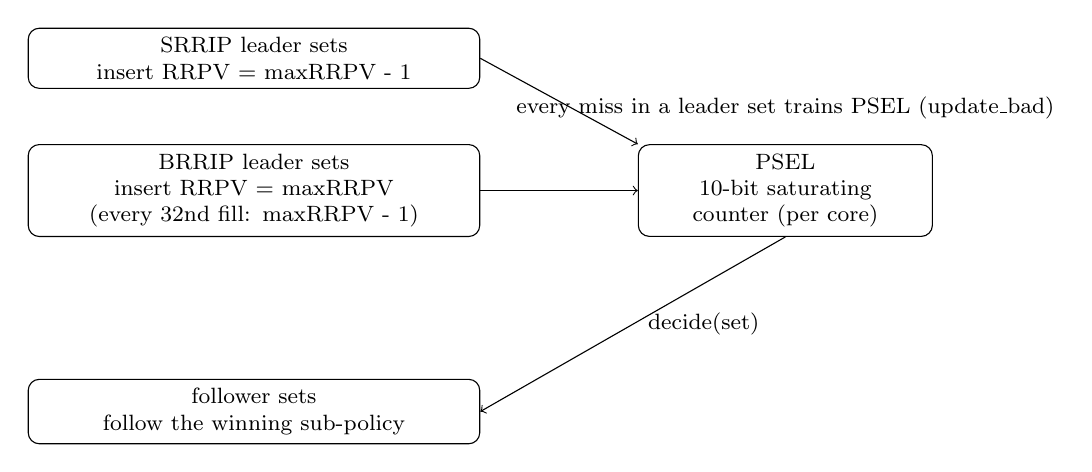
\begin{tikzpicture}[every node/.style={font=\footnotesize}, node distance=0.7cm]
\node[draw, rounded corners, text width=5.5cm, align=center] (srrip)
  {\lr{SRRIP leader sets} \\ \lr{insert RRPV = maxRRPV - 1}};
\node[draw, rounded corners, text width=5.5cm, align=center, below=of srrip] (brrip)
  {\lr{BRRIP leader sets} \\ \lr{insert RRPV = maxRRPV} \\ \lr{(every 32nd fill: maxRRPV - 1)}};
\node[draw, rounded corners, text width=5.5cm, align=center, below=1.8cm of brrip] (foll)
  {\lr{follower sets} \\ \lr{follow the winning sub-policy}};
\node[draw, rounded corners, text width=3.5cm, align=center, right=2cm of brrip] (psel)
  {\lr{PSEL} \\ \lr{10-bit saturating counter (per core)}};
\draw[->] (srrip.east) -- (psel.north west);
\draw[->] (brrip.east) -- (psel.west);
\draw[->] (psel.south) -- node[right, xshift=2pt] {\lr{decide(set)}} (foll.east);
\node[above=0.2cm of psel, align=center] {\lr{every miss in a leader set trains PSEL (update\_bad)}};
\end{tikzpicture}
\caption{سازوکار \lr{set-dueling} و نقش شمارنده ی \lr{PSEL} در \lr{DRRIP}],
  \{
    import cetz.draw: *

    let cell(x0, y0, x1, y1, name, body, fill) = \{
      rect((x0, y0), (x1, y1), name: name, fill: fill, stroke: 0.6pt + rule-color, radius: 2pt)
      content(((x0 + x1) / 2, (y0 + y1) / 2), align(center, body))
    \}

    cell(0, 4.5, 7.2, 5.9, "srrip", [SRRIP leader sets \textbackslash{} insert RRPV = maxRRPV - 1], accent.transparentize(82\%))
    cell(0, 2.5, 7.2, 4.1, "brrip", [BRRIP leader sets \textbackslash{} insert RRPV = maxRRPV \textbackslash{} (every 32nd fill: maxRRPV - 1)], accent.transparentize(82\%))
    cell(0, 0.3, 7.2, 1.7, "foll", [follower sets \textbackslash{} follow the winning sub-policy], surface)
    cell(9.0, 2.6, 13.4, 4.6, "psel", [PSEL \textbackslash{} 10-bit saturating \textbackslash{} counter (per core)}
\end{figure}

نحوه ی بروزرسانی اطلاعات پس از برخورد (\lr{hit}):

مستقل از اینکه \lr{set} از نوع \lr{leader} است یا \lr{follower} و مستقل از اینکه کدام \lr{sub-policy} فعال است، مقدار \lr{RRPV} بلوکی که \lr{hit} شده به ۰ ریست می شود. برای دسترسی های \lr{WRITE} به جای ۰ مقدار \lr{\texttt{maxRRPV - 1}} گذاشته می شود تا \lr{writeback} باعث نشود بلوکی الکی امن به حساب بیاید. نکته ی مهم دیگر این است که در مسیر \lr{hit} شمارنده ی \lr{PSEL} دست نمی خورد و آموزش \lr{PSEL} فقط از روی \lr{miss} ها انجام می شود.

نحوه ی بروزرسانی اطلاعات پس از جایگزینی (\lr{fill}):

اول مثل \lr{SRRIP}، در \lr{\texttt{find\_victim}} مقدار \lr{RRPV} همه ی بلوک های \lr{set} به اندازه ی لازم زیاد می شود تا قربانی با مقدار بیشینه پیدا شود. بعد از درج بلوک جدید، تابع \lr{\texttt{decide(set)}} مشخص می کند کدام \lr{sub-policy} اجرا شود: \lr{set} های \lr{leader} همیشه سیاست ثابت خودشان (\lr{SRRIP} یا \lr{BRRIP}) و \lr{set} های \lr{follower} بر اساس مقدار فعلی \lr{PSEL}. در حالت \lr{SRRIP} مقدار \lr{\texttt{maxRRPV - 1}} و در حالت \lr{BRRIP} مقدار \lr{\texttt{maxRRPV}} داده می شود، به جز یک بار در هر ۳۲ درج که به صورت چرخشی مقدار \lr{\texttt{maxRRPV - 1}} می گیرد.

سپس برای خود \lr{PSEL} داریم: در پایان هر \lr{fill} تابع \lr{\texttt{update\_bad(set)}} صدا زده می شود. چون \lr{fill} فقط بعد از \lr{miss} اتفاق می افتد، هر \lr{miss} در یک \lr{set} رهبر شمارنده را به ضرر سیاست همان رهبر حرکت می دهد و بعد از مدتی \lr{PSEL} به سمت سیاستی می رود که در \lr{set} های نمونه \lr{miss} کمتری داشته است. این تنها بخش واقعا پویای این روش است (شمارنده ی \lr{PSEL} از روی \lr{set} های \lr{leader} یاد می گیرد و مثل دیکتاتور به \lr{set} های \lr{follower} غالب می کند).

شرایط عملکرد مناسب و نامناسب:

سیاست \lr{DRRIP} تقریبا در همه ی شرایط خوب عمل می کند چون به صورت پویا بین دو روش جابه جا می شود. صرفا در جاهایی ممکن است بد عمل کند که \lr{working set} اینقدر کم باشد که روش فرصت یادگیری نداشته باشد و \lr{overkill} باشد.

نکات کد:

\subsubsection{قطعه ۱ — ثابت ها و شمارنده ی \lr{PSEL}}

\begin{latin}
\begin{lstlisting}
struct drrip : public champsim::modules::replacement {
  static constexpr unsigned maxRRPV = 3;
  static constexpr unsigned BRRIP_MAX = 32;
  static constexpr unsigned PSEL_WIDTH = 10;

  enum class set_type { follower, brrip_leader, srrip_leader };

  unsigned brrip_counter;

  std::vector<unsigned> rrpv;
  std::vector<champsim::msl::dscounter<long, PSEL_WIDTH>> PSEL;
};

drrip::drrip(CACHE* cache)
    : replacement(cache), NUM_SET(cache->NUM_SET), NUM_WAY(cache->NUM_WAY),
      rrpv(static_cast<std::size_t>(NUM_SET * NUM_WAY)),
      PSEL(NUM_CPUS, champsim::msl::dscounter<long, PSEL_WIDTH>(champsim::msl::get_sample_rate(NUM_SET)))
{
}
\end{lstlisting}
\end{latin}

یک شمارنده ی \lr{PSEL} با طول ۱۰ بیت به ازای هر هسته داریم. ۳ دسته برای \lr{set} ها طبق توضیحی که دادیم داریم. و بقیه ی المان های \lr{SRRIP} و المان های مشابه \lr{BIP} را نیز مشاهده می کنیم.

\subsubsection{قطعه ۲ — دو \lr{sub-policy} درج}

\begin{latin}
\begin{lstlisting}
void drrip::update_brrip(long set, long way)
{
  get_rrpv(set, way) = maxRRPV;

  brrip_counter++;
  if (brrip_counter == BRRIP_MAX) {
    brrip_counter = 0;
    get_rrpv(set, way) = maxRRPV - 1;
  }
}

void drrip::update_srrip(long set, long way) { get_rrpv(set, way) = maxRRPV - 1; }
\end{lstlisting}
\end{latin}

در حالت \lr{BRRIP} بلوک جدید در ۳۱ حالت از هر ۳۲ حالت با مقدار \lr{\texttt{maxRRPV}} اضافه می شود (اینجا یک تفاوت ریز با \lr{BIP} دارد و آن این است که در \lr{BIP} این موضوع رندوم بود ولی اینجا به صورت چرخشی و سیکلی است و رندوم نیست، تاثیر عملکردی آن شاید ناچیز باشد و تقریبا یکسان باشند ولی از لحاظ سخت افزاری خیلی ساده تر از رندوم است)، یعنی در مرز خروج قرار می گیرد و اگر تا اولین جست وجوی قربانی استفاده نشود بیرون می رود. فقط یک بار در هر ۳۲ درج، مقدار \lr{\texttt{maxRRPV - 1}} داده می شود تا \lr{cache} بتواند به تدریج محتوای جدید را نگه دارد.

تابع \lr{\texttt{update\_srrip}} دقیقا همان درج \lr{SRRIP} است و هیچ تفاوتی با آن ندارد.

\subsubsection{قطعه ۳ — انتخاب \lr{sub-policy} در زمان درج}

\begin{latin}
\begin{lstlisting}
void drrip::replacement_cache_fill(uint32_t triggering_cpu, long set, long way, ...)
{
  // do not update replacement state for writebacks
  if (access_type{type} == access_type::WRITE) {
    get_rrpv(set, way) = maxRRPV - 1;
    return;
  }
  if (PSEL[triggering_cpu].decide(set)) {
    update_brrip(set, way);
  } else {
    update_srrip(set, way);
  }
  // cache miss, update bad
  PSEL[triggering_cpu].update_bad(set);
}
\end{lstlisting}
\end{latin}

تابع \lr{\texttt{decide(set)}} برای \lr{set} های \lr{leader} همیشه سیاست فیکس شده ی خودشان را برمی گرداند و برای \lr{set} های \lr{follower} بر اساس مقدار فعلی \lr{PSEL} تصمیم می گیرد.

تابع \lr{\texttt{update\_bad(set)}} در هر \lr{fill} صدا زده می شود و چون \lr{fill} فقط بعد از \lr{miss} اتفاق می افتد، عملا هر \lr{miss} در یک \lr{set} رهبر، \lr{PSEL} را به ضرر سیاست همان رهبر تغییر می دهد. در نتیجه بعد از مدتی \lr{PSEL} به سمت سیاستی می رود که در \lr{set} های نمونه \lr{miss} کمتری داده است. این همان بخش پویای این روش است. اینکه خود تابع \lr{\texttt{update\_bad}} چطوری پیاده سازی شده است در فایل های داخلی \lr{ChampSim} است و خیلی جزیی می شود.

\subsubsection{قطعه ۴ — \lr{hit} و انتخاب قربانی}

\begin{latin}
\begin{lstlisting}
void drrip::update_replacement_state(..., uint8_t hit)
{
  if (hit) {
    if (access_type{type} == access_type::WRITE) {
      get_rrpv(set, way) = maxRRPV - 1;
      return;
    }
    get_rrpv(set, way) = 0; // DRRIP always promotes a cache line to the MRU position
  }
}

long drrip::find_victim(uint32_t triggering_cpu, uint64_t instr_id, long set, ...)
{
  auto begin = std::next(std::begin(rrpv), set * NUM_WAY);
  auto end = std::next(begin, NUM_WAY);

  auto victim = std::max_element(begin, end);
  if (auto rrpv_update = maxRRPV - *victim; rrpv_update != 0)
    for (auto it = begin; it != end; ++it)
      *it += rrpv_update;

  return std::distance(begin, victim);
}
\end{lstlisting}
\end{latin}

تابع \lr{\texttt{find\_victim}} از نظر منطقی دقیقا همان \lr{SRRIP} است و فقط به جای \lr{\texttt{std::transform}} از یک حلقه استفاده کرده است.

در زمان برخورد، بدون توجه به اینکه کدام \lr{sub-policy} فعال است، مقدار \lr{RRPV} به ۰ می رسد.

\subsection{\lr{SHiP}}

منطق انتخاب بلوک قربانی:

در روش \lr{SHiP} (\lr{Signature-based Hit Predictor})، کاملا مشابه روش \lr{SRRIP} مقادیر \lr{RRPV} به ازای هر بلوک داریم که دقیقا به همان روش \lr{SRRIP} بلوک هدف را خارج می کنیم.

نحوه بروزرسانی اطلاعات کمکی:

در این \lr{policy} ما روی مقدار اولیه \lr{RRPV} که به ازای هر بلوک نسبت می دهیم خلاقیت به خرج می دهیم و سعی می کنیم مقدار هوشمندانه ای برای آن تعیین کنیم. به این صورت که در کنار \lr{RRPV} یک تگ به اسم \lr{signature} هم به هر بلوک هنگام اضافه شدن به \lr{set} به آن می دهیم که بر اساس ناحیه ی حافظه ای است که در آن قرار داشته است یا آدرس حافظه مربوط به آن است (\lr{PC}) (کلا قرارداد مخصوص به خود دارد، مثلا در کد ما همان \lr{PC} است). یک جدول به اسم \lr{SHCT} (\lr{Signature History Counter Table}) نگه می داریم که به ازای هر \lr{signature} یک شمارنده دارد که در هر بار دسترسی به بلوک با ان \lr{signature} خاص شمارنده مربوط به \lr{signature} در جدول کم می شود. عملا مقدار به ازای هر \lr{signature} در این جدول بیان می کند که این پترن خاص از حافظه چقدر امکان مجدد بازخواست و دسترسی دارند. هنگام اضافه کردن بلوک به \lr{set} از این جدول \lr{lookup} انجام می دهیم و مقدار مربوط به \lr{signature} این بلوک را می خوانیم، بر اساس این مقدار \lr{RRPV} را مقداردهی می کنیم. در صورتی که این مقدار کم باشد و یعنی احتمال بازخواست این \lr{signature} زیاد باشد مقدار \lr{RRPV} آن را یک چیز کم مثل ۰ یا ۱ می دهیم (البته اینکه در حالت خوب یک مقدار \lr{RRPV} به آن داده شود در کد نیست و در اولین پیاده سازی های این ایده هم ظاهرا نبوده و در مقالات و ورژن های بعدی که بهبود یافته است ظاهر می شود). و اگر مقدار جدول زیاد باشد و یعنی این \lr{signature} احتمالا زیاد بازخواست نمی شود مقدار \lr{RRPV} بالایی مثل \lr{\texttt{MAX\_RRPV}} به آن نسبت می دهیم.

در هنگام \lr{hit} مقدار \lr{RRPV} بلوک به ۰ ریست می شود و ورودی داخل جدول \lr{SHCT} که مربوط به \lr{signature} این بلوک است یکی کم می شود.

در هنگامی که بلوک بدون اینکه یکبار هم \lr{hit} شده باشد در جدول مقدار مربوط به \lr{signature} آن یکی زیاد می شود.

نکته ی بسیار مهم این است که این جدول اگر برای تمام \lr{set} های موجود ذخیره شود سخت افزار خیلی بزرگی می خواهد، پس به جای اینکار ما این را برای تعداد محدودی \lr{set} انجام می دهیم و به بقیه \lr{set} ها تعمیم می دهیم. به این \lr{sampler} می گوییم که چیزی شبیه شبکه عصبی که با یک سری \lr{set} ها \lr{train} می شود و روی بقیه تست می شود. به این شکل سخت افزار کمتری مصرف می شود. در جاهای مختلف کد این موضوع تکرار شده ولی چون از توضیحی که دادیم خارج نیست، فرض می کنیم کلا \lr{sampler} را ندید می گیریم و کلی توضیح می دهیم، پس داخل کد و توضیحات بیشتر جاها منظورمان خود \lr{sampler} است که در یادگیری استفاده می شود ولی برای ساده سازی به خود جدول اشاره کردیم.

\begin{figure}[H]
\centering
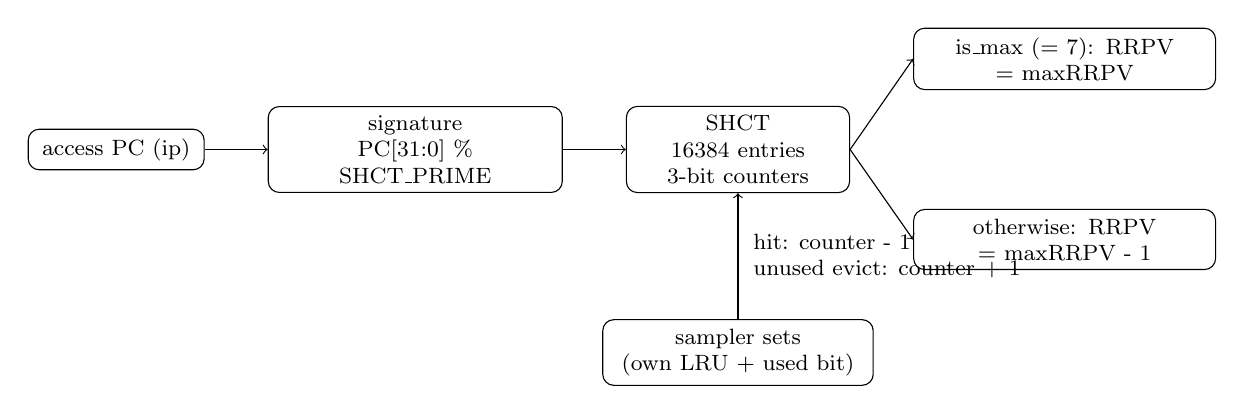
\begin{tikzpicture}[every node/.style={font=\footnotesize}, node distance=0.8cm]
\node[draw, rounded corners, text width=2cm, align=center] (pc) {\lr{access PC (ip)}};
\node[draw, rounded corners, text width=3.5cm, align=center, right=of pc] (sig)
  {\lr{signature} \\ \lr{PC[31:0] \% SHCT\_PRIME}};
\node[draw, rounded corners, text width=2.6cm, align=center, right=of sig] (shct)
  {\lr{SHCT} \\ \lr{16384 entries} \\ \lr{3-bit counters}};
\node[draw, rounded corners, text width=3.6cm, align=center, above right=0.2cm and 0.8cm of shct] (bad)
  {\lr{is\_max (= 7): RRPV = maxRRPV}};
\node[draw, rounded corners, text width=3.6cm, align=center, below right=0.2cm and 0.8cm of shct] (good)
  {\lr{otherwise: RRPV = maxRRPV - 1}};
\node[draw, rounded corners, text width=3.2cm, align=center, below=1.6cm of shct] (samp)
  {\lr{sampler sets} \\ \lr{(own LRU + used bit)}};
\draw[->] (pc) -- (sig);
\draw[->] (sig) -- (shct);
\draw[->] (shct.east) -- (bad.west);
\draw[->] (shct.east) -- (good.west);
\draw[->] (samp.north) -- node[right, xshift=2pt, align=left]
  {\lr{hit: counter - 1} \\ \lr{unused evict: counter + 1}} (shct.south);
\end{tikzpicture}
\caption{مسیر پیش بینی و مسیر آموزش جدول \lr{SHCT} در \lr{SHiP}],
  length: 0.82cm,
  \{
    import cetz.draw: *

    let cell(x0, y0, x1, y1, name, body, fill) = \{
      rect((x0, y0), (x1, y1), name: name, fill: fill, stroke: 0.6pt + rule-color, radius: 2pt)
      content(((x0 + x1) / 2, (y0 + y1) / 2), align(center, body))
    \}

    cell(0, 4.2, 3.0, 5.6, "pc", [access PC \textbackslash{} (ip)], surface)
    cell(4.0, 4.2, 9.0, 5.6, "sig", [signature \textbackslash{} PC[31:0] \% SHCT\_PRIME], surface)
    cell(10.0, 3.9, 14.0, 5.9, "shct", [SHCT \textbackslash{} 16384 entries \textbackslash{} 3-bit counters], accent.transparentize(82\%))
    cell(15.0, 5.0, 20.6, 6.2, "bad", [is\_max (= 7): \textbackslash{} RRPV = maxRRPV], surface)
    cell(15.0, 3.4, 20.6, 4.6, "good", [otherwise: \textbackslash{} RRPV = maxRRPV - 1], surface)
    cell(9.2, 0.4, 14.8, 1.8, "samp", [sampler sets \textbackslash{} (own LRU + used bit)], surface)

    line("pc.east", "sig.west", mark: (end: ">"), stroke: 0.6pt + accent)
    line("sig.east", "shct.west", mark: (end: ">"), stroke: 0.6pt + accent)
    line("shct.east", "bad.west", mark: (end: ">"), stroke: 0.6pt + accent)
    line("shct.east", "good.west", mark: (end: ">"), stroke: 0.6pt + accent)
    line("samp.north", "shct.south", mark: (end: ">"), stroke: 0.6pt + accent)

    content((17.8, 2.4), align(center)[insertion RRPV \textbackslash{} of the new block])
    content((11.7, 2.85), align(right)[hit: counter - 1 \textbackslash{} unused evict: counter + 1], anchor: "east")
    content((8.8, 1.1), align(right)[only sampled sets \textbackslash{} train the table}
\end{figure}

نحوه ی بروزرسانی اطلاعات پس از برخورد (\lr{hit}):

ابتدا در کش اصلی مقدار \lr{RRPV} آن بلوک مثل \lr{SRRIP} به ۰ ریست می شود و سپس برای \lr{train} اگر \lr{set} مورد نظر جزو \lr{set} های \lr{sampler} باشد، خانه ی متناظر در جدول \lr{SHCT} پیدا می شود و مقدار آن یکی کم می شود، چون این \lr{hit} ثابت می کند که آن \lr{signature} (یعنی همان \lr{PC}) داده ای می آورد که واقعا دوباره استفاده می شود. همچنین بیت \lr{\texttt{used}} آن خانه ی \lr{sampler} برابر \lr{\texttt{true}} می شود تا بعدا موقع خروج، این بلوک به عنوان «بدرد نخور» جریمه نشود. اگر \lr{set} جزو نمونه ها نباشد هیچ \lr{train} ای انجام نمی شود و فقط \lr{RRPV} ریست می شود.

نحوه ی بروزرسانی اطلاعات پس از جایگزینی (\lr{fill}):

ابتدا \lr{signature} بلوک جدید از ۳۲ بیت پایین \lr{PC} ساخته و با \lr{\texttt{\% SHCT\_PRIME}} روی جدول مپ می شود و مقدار آن خانه خوانده می شود. اگر شمارنده به بیشینه رسیده باشد (\lr{\texttt{is\_max}}، یعنی مقدار ۷) بلوک با \lr{\texttt{maxRRPV}} درج می شود که یعنی همان لحظه در مرز خروج است، وگرنه مقدار پیشفرض \lr{\texttt{maxRRPV - 1}} مثل \lr{SRRIP} را می گیرد. برای دسترسی های \lr{WRITE} هم بدون هیچ \lr{lookup} ای همان مقدار امن \lr{\texttt{maxRRPV - 1}} گذاشته می شود.

سپس برای \lr{train} وقتی در یک \lr{set} نمونه یک خانه ی \lr{sampler} بازنویسی می شود، اگر آن خانه بیت \lr{\texttt{used}} نداشته باشد یعنی بلوک قبلی بدون حتی یک بار استفاده خارج شده است، پس شمارنده ی مربوط به \lr{signature} آن یکی زیاد می شود. بعد خانه با آدرس و \lr{PC} جدید مقداردهی و \lr{\texttt{used}} دوباره صفر می شود. توجه کنیم که \lr{sampler} برای خودش یک سیاست \lr{LRU} مستقل با \lr{\texttt{last\_used}} دارد که هیچ ربطی به \lr{RRPV} های کش اصلی ندارد.

شرایط عملکرد مناسب و نامناسب:

سیاست \lr{SHiP} وقتی بهترین عملکرد را دارد که پترن استفاده ی برنامه از یک سری خانه های حافظه مشخص و الگودار باشد؛ \lr{SHiP} می تواند این الگو ها را تشخیص بدهد و از آنها استفاده بکند (عملا استفاده های مجدد از یک سری از خانه های حافظه معنی دار و الگو دار باشند).

چون \lr{SHiP} به مرور یاد می گیرد و جدول \lr{SHCT} را باید پر کند، فرآیند یادگیری آن کمی طول می کشد و به همین دلیل در اوایل شاید خوب عمل نکند. همچنین وقتی که پترن و جنس الگوی دسترسی برنامه عوض می شود، چون جدول هنوز روی پترن قبلی یاد گرفته، اوایل خوب عمل نمی کند و بندری می زند.

نکات کد:

\subsubsection{قطعه ۱ — ساختار \lr{sampler} و جدول \lr{SHCT}}

\begin{latin}
\begin{lstlisting}
struct ship : public champsim::modules::replacement {
  static constexpr int maxRRPV = 3;
  static constexpr std::size_t SHCT_SIZE = 16384;
  static constexpr unsigned SHCT_PRIME = 16381;
  static constexpr unsigned SHCT_MAX = 7;

  class SAMPLER_class
  {
  public:
    bool valid = false;
    bool used = false;
    champsim::address address{};
    champsim::address ip{};
    uint64_t last_used = 0;
  };

  std::vector<SAMPLER_class> sampler;
  std::vector<int> rrpv_values;
  champsim::msl::categorizer<long> set_categorizer;
  champsim::data::bits sampler_tag_bits;

  std::vector<std::array<champsim::msl::fwcounter<champsim::msl::lg2(SHCT_MAX + 1)>, SHCT_SIZE>> SHCT;
};
\end{lstlisting}
\end{latin}

ساختار داده \lr{SHCT} یک جدول با ۱۶۳۸۴ خانه است که هر خانه ی آن یک شمارنده ۳ بیتی است (چون \lr{\texttt{SHCT\_MAX = 7}} است).

هر خانه ی \lr{sampler} یک بیت \lr{\texttt{used}} دارد که می گوید آیا آن بلوک بعد از درج حداقل یک بار استفاده شد یا نه.

\subsubsection{قطعه ۲ — آموزش جدول از روی \lr{sampler}}

\begin{latin}
\begin{lstlisting}
void ship::update_replacement_state(..., uint8_t hit)
{
  // update sampler
  if (set_categorizer.get_sample_category(set) == 0) {
    auto s_idx = set / champsim::msl::get_sample_rate(NUM_SET);
    auto s_set_begin = std::next(std::begin(sampler), s_idx * NUM_WAY + ...);
    auto s_set_end = std::next(s_set_begin, NUM_WAY);

    // check hit
    auto match = std::find_if(s_set_begin, s_set_end, [addr = full_addr, shamt = sampler_tag_bits](auto x) {
      return x.valid && x.address.slice_upper(shamt) == addr.slice_upper(shamt);
    });
    if (match != s_set_end) {
      auto SHCT_idx = match->ip.slice_lower<32_b>().to<std::size_t>() % SHCT_PRIME;
      SHCT[triggering_cpu][SHCT_idx] -= 1;
      match->used = true;
    } else {
      match = std::min_element(s_set_begin, s_set_end, [](auto x, auto y) { return x.last_used < y.last_used; });

      if (!match->used) {
        auto SHCT_idx = match->ip.slice_lower<32_b>().to<std::size_t>() % SHCT_PRIME;
        SHCT[triggering_cpu][SHCT_idx] += 1;
      }

      match->valid = true;
      match->address = full_addr;
      match->ip = ip;
      match->used = false;
    }

    // update LRU state
    match->last_used = access_count++;
  }

  if (hit)
    get_rrpv(set, way) = 0;
}
\end{lstlisting}
\end{latin}

در صورتی که \lr{hit} داشته باشیم از شمارنده مربوط به آن \lr{signature} یکی کم می شود و اگر بدون اینکه از بلوک اضافه شده استفاده ی مجدد شود و \lr{evict} شود شمارنده را یکی زیاد می کنیم.

بخش \lr{signature} همان ۳۲ بیت پایین \lr{PC} است که با \lr{\texttt{\% SHCT\_PRIME}} روی جدول مپ می شود.

بخش \lr{sampler} برای خودش یک سیاست \lr{LRU} مستقل دارد که با \lr{\texttt{last\_used}} و \lr{\texttt{access\_count}} پیاده شده و هیچ ربطی به \lr{RRPV} های کش اصلی ندارد. یعنی \lr{sampler} یک کش مجازی کوچک است که فقط برای آموزش نگه داشته می شود.

در صورت \lr{hit} در \lr{cache} مقدار \lr{RRPV} را به ۰ ریست می کند.

\subsubsection{قطعه ۳ — استفاده از پیش بینی در زمان درج}

\begin{latin}
\begin{lstlisting}
void ship::replacement_cache_fill(uint32_t triggering_cpu, long set, long way, ...)
{
  // handle writeback access
  if (access_type{type} == access_type::WRITE) {
    get_rrpv(set, way) = maxRRPV - 1;
    return;
  }

  // SHIP prediction
  auto SHCT_idx = ip.slice_lower<32_b>().to<std::size_t>() % SHCT_PRIME;

  get_rrpv(set, way) = maxRRPV - 1;
  if (SHCT[triggering_cpu][SHCT_idx].is_max())
    get_rrpv(set, way) = maxRRPV;
}
\end{lstlisting}
\end{latin}

همان بخش پویا که بر اساس مقدار جدول تصمیم می گیرد که مقدار اولیه \lr{RRPV} چه باشد. حالت پیشفرض مثل \lr{SRRIP} مقدار \lr{\texttt{maxRRPV - 1}} است و حالت خیلی بد مقدار \lr{\texttt{maxRRPV}} را به خود می گیرد.

شرط \lr{\texttt{is\_max}} همان بررسی حالت خیلی بد است که در صورتی که شمارنده پر شده باشد (یعنی مقدار ۷ را به خود گرفته باشد) فعال می شود.

\subsubsection{قطعه ۴ — انتخاب قربانی}

\begin{latin}
\begin{lstlisting}
long ship::find_victim(uint32_t triggering_cpu, uint64_t instr_id, long set, ...)
{
  auto begin = std::next(std::begin(rrpv_values), set * NUM_WAY);
  auto end = std::next(begin, NUM_WAY);

  auto victim = std::max_element(begin, end);
  if (auto rrpv_update = maxRRPV - *victim; rrpv_update != 0)
    for (auto it = begin; it != end; ++it)
      *it += rrpv_update;

  return std::distance(begin, victim);
}
\end{lstlisting}
\end{latin}

این تابع عینا همان \lr{\texttt{find\_victim}} سیاست های \lr{SRRIP} و \lr{DRRIP} است.

\newpage
\section{مقایسه ی سیاست ها روی ردپا ها}

برای تعیین عملکرد هر سیاست، از معیار \lr{IPC} استفاده شده است. چرا که در نهایت، افزایش سرعت کلی برنامه را دقیق تر از معیار های دیگری نظیر \lr{Hit rate} نشان می دهد.

\subsection{سوال ۱: عملکرد میانگین هر سیاست}

عملکرد میانگین هر سیاست در میان همه ی ردپا ها و همه ی تعداد \lr{set} ها به این صورت است:

\begin{table}[H]
\centering
\begin{tabular}{|c|c|c|}
\hline
\lr{Strategy} & \lr{Average IPC} & \lr{Average IPC/LRU} \\
\hline
\lr{bip} & \lr{0.3799} & \lr{1.0269} \\
\hline
\lr{drrip} & \lr{0.3789} & \lr{1.0244} \\
\hline
\lr{fifo} & \lr{0.3685} & \lr{0.9962} \\
\hline
\lr{lru} & \lr{0.3699} & \lr{1.0000} \\
\hline
\lr{mru} & \lr{0.3630} & \lr{0.9813} \\
\hline
\lr{random} & \lr{0.3720} & \lr{1.0057} \\
\hline
\lr{ship} & \lr{0.3807} & \lr{1.0292} \\
\hline
\lr{srrip} & \lr{0.3769} & \lr{1.0189} \\
\hline
\end{tabular}
\caption{میانگین \lr{IPC} هر سیاست روی همه ی ردپا ها و همه ی اندازه های کش}
\end{table}

که این مقادیر بسیار به هم نزدیک هستند. دلیل این اتفاق این است که تاثیر کش های لایه های بالاتر و باقی سخت افزار پردازنده بسیار بیشتر از تاثیر صرفا کش لایه ی آخر در سرعت کلی برنامه است. طبق این آمار، سیاست \lr{ship} با بیشترین مقدار میانگین \lr{IPC}، در میانگین همه ی ردپا ها بهترین عملکرد را داشته است.

\subsection{سوال ۲: آیا یک سیاست ثابت در همه ی ردپا ها بهترین است؟}

با توجه به نمودار های \lr{IPC}، مثلا در ردپای \lr{mcf}، سیاست های \lr{ship} و \lr{srrip} و \lr{bip} بهترین عملکرد را دارند. ولی \lr{ship} در ردپای \lr{gcc} عملکرد بسیار پایینی دارد. همچنین \lr{srrip} و \lr{bip} در ردپا های \lr{lbm} و \lr{omnetpp} عملکرد جالبی ندارند. پس می توان نتیجه گرفت هیچ سیاست ثابتی بین آنهایی که بررسی شدند وجود ندارد که در همه ی ردپا ها بهترین باشد.

\subsection{سوال ۳: مقایسه ی سیاست های پیشرفته با \lr{LRU}}

با بررسی نمودار ها، می توان گفت در ردپای \lr{gcc}، همه ی سیاست های پیشرفته (\lr{ship} و \lr{srrip} و \lr{drrip} و \lr{bip}) بهتر از \lr{lru} عمل کرده اند. در مورد ردپای \lr{lbm} می توان گفت که عملکرد سیاست های مختلف به شدت به تعداد \lr{set} ها وابسته بوده. به طوری که در تعداد کمتر آن (حدود ۱۰۲۴ یا ۲۰۴۸ \lr{set}) تفاوت معناداری بین سیاست های پیشرفته ی \lr{ship} و \lr{srrip} و \lr{drrip} با \lr{lru} وجود ندارد و صرفا سیاست \lr{bip} بوده که بسیار بهتر از آن عمل کرده است. اما در تعداد \lr{set} های بیشتر (مثلا ۴۰۹۶)، فقط عملکرد \lr{ship} و \lr{drrip} به طور قابل ملاحظه ای بیشتر از \lr{lru} است. در مورد ردپای \lr{mcf}، باز هم همه ی سیاست های پیشرفته از \lr{lru} بهتر عمل کرده اند؛ صرفا \lr{drrip} در تعداد \lr{set} های پایین مقداری کمتر از بقیه عمل می کند. در نهایت در ردپای \lr{omnetpp} می توان گفت که هیچ سیاست پیشرفته ای چندان بهتر از \lr{lru} عمل نکرده است، مگر در تعداد \lr{set} های پایینتر (حدود ۱۰۲۴) که باز هم تفاوت خیلی زیادی ندارند.

\subsection{سوال ۴: کجا \lr{LRU} و \lr{FIFO} کفایت می کنند؟}

با توجه به بخش قبلی و نیز نمودار ها می توان نتیجه گرفت که فقط در ردپای \lr{omnetpp}، دو سیاست \lr{lru} و \lr{fifo} کفایت می کنند و عملکرد بسیار خوبی دارند.

\subsection{سوال ۵: آیا کاهش \lr{Miss Rate} همیشه به افزایش \lr{IPC} منجر می شود؟}

نه لزوما. اگرچه معمولا کاهش \lr{Miss Rate} باعث افزایش \lr{IPC} می شود، اما رابطه کاملا خطی نیست. برای مثال \lr{SHiP} در بعضی ردپا ها نرخ \lr{Miss} کمتری نسبت به \lr{LRU} دارد ولی افزایش \lr{IPC} آن بسیار اندک است. در بعضی موارد نیز اختلاف زیاد در \lr{Miss Rate} تنها به افزایش جزیی \lr{IPC} منجر شده است. دلیل آن این است که \lr{IPC} علاوه بر کش، به عواملی مانند وابستگی های داده، پیش بینی انشعاب، اجرای موازی دستور ها، و سایر \lr{stall} های پردازنده نیز وابسته است. بنابراین کاهش \lr{Miss Rate} شرط لازم برای افزایش \lr{IPC} است، اما همیشه شرط کافی نیست.

\subsection{سوال ۶: رفتار سیاست های تطبیقی}

سیاست هایی مانند \lr{BIP} و \lr{DRRIP} و \lr{SHiP} تلاش می کنند رفتار برنامه را هنگام اجرا تشخیص داده و خود را با آن تطبیق دهند. در ردپا هایی مانند \lr{mcf} و \lr{lbm} این سیاست ها توانسته اند خطوط مفید را مدت بیشتری در کش نگه دارند و از جایگزینی زودهنگام جلوگیری کنند؛ در نتیجه هم نرخ \lr{Miss} کاهش یافته و هم \lr{IPC} افزایش یافته است.

در \lr{omnetpp}، الگوی دسترسی از قبل با رفتار \lr{LRU} سازگار بوده است؛ بنابراین سازوکار های تطبیقی سودی نداشته و حتی سربار تصمیم گیری باعث افت جزیی عملکرد می شود.

با بزرگ تر شدن اندازه ی کش (از ۱۰۲۴ به ۴۰۹۶ \lr{set})، مزیت سیاست های تطبیقی در ردپا های ظرفیت محور مانند \lr{mcf} بیشتر نمایان شده است، زیرا فضای بیشتر کش امکان استفاده ی بهتر از تصمیم های هوشمندانه را فراهم کرده است.

\subsection{نمودار ها}

در این بخش تمام نمودار هایی که تحلیل های بالا بر اساس آنها نوشته شده اند را کنار هم آورده ایم. هر دو دسته هر سه اندازه ی کش (۱۰۲۴ و ۲۰۴۸ و ۴۰۹۶ \lr{set}) را پوشش می دهند و فقط در اینکه چه چیزی روی محور افقی است با هم فرق دارند.

\subsubsection{مقایسه بر حسب سیاست، برای هر سه اندازه ی کش}

در این دسته محور افقی سیاست جایگزینی است و هر منحنی مربوط به یکی از سه اندازه ی کش (۱۰۲۴ و ۲۰۴۸ و ۴۰۹۶ \lr{set}) است، پس اثر خود سیاست را در اندازه های مختلف نشان می دهد.

\begin{figure}[H]
\centering
\begin{latin}

\includegraphics[width=0.47\textwidth]{{figures/policy_on_x/403.gcc-17B_ipc}.png} \hfill 
\includegraphics[width=0.47\textwidth]{{figures/policy_on_x/403.gcc-17B_hit_rate}.png}
\end{latin}
\caption{ردپای \lr{403.gcc}: \lr{IPC} و نرخ برخورد بر حسب سیاست، برای هر سه اندازه ی کش}
\end{figure}

\begin{figure}[H]
\centering
\begin{latin}

\includegraphics[width=0.47\textwidth]{{figures/policy_on_x/429.mcf-51B_ipc}.png} \hfill 
\includegraphics[width=0.47\textwidth]{{figures/policy_on_x/429.mcf-51B_hit_rate}.png}
\end{latin}
\caption{ردپای \lr{429.mcf}: \lr{IPC} و نرخ برخورد بر حسب سیاست، برای هر سه اندازه ی کش}
\end{figure}

\begin{figure}[H]
\centering
\begin{latin}

\includegraphics[width=0.47\textwidth]{{figures/policy_on_x/470.lbm-1274B_ipc}.png} \hfill 
\includegraphics[width=0.47\textwidth]{{figures/policy_on_x/470.lbm-1274B_hit_rate}.png}
\end{latin}
\caption{ردپای \lr{470.lbm}: \lr{IPC} و نرخ برخورد بر حسب سیاست، برای هر سه اندازه ی کش}
\end{figure}

\begin{figure}[H]
\centering
\begin{latin}

\includegraphics[width=0.47\textwidth]{{figures/policy_on_x/471.omnetpp-188B_ipc}.png} \hfill 
\includegraphics[width=0.47\textwidth]{{figures/policy_on_x/471.omnetpp-188B_hit_rate}.png}
\end{latin}
\caption{ردپای \lr{471.omnetpp}: \lr{IPC} و نرخ برخورد بر حسب سیاست، برای هر سه اندازه ی کش}
\end{figure}

\subsubsection{مقایسه بر حسب تعداد \lr{set}}

در این دسته محور افقی تعداد \lr{set} هاست و هر منحنی مربوط به یک سیاست است، پس نشان می دهد هر سیاست با بزرگ تر شدن کش چطور رفتار می کند.

\begin{figure}[H]
\centering
\begin{latin}

\includegraphics[width=0.47\textwidth]{{figures/size_on_x/403.gcc-17B_ipc}.png} \hfill 
\includegraphics[width=0.47\textwidth]{{figures/size_on_x/403.gcc-17B_hit_rate}.png}
\end{latin}
\caption{ردپای \lr{403.gcc}: \lr{IPC} و نرخ برخورد بر حسب تعداد \lr{set}}
\end{figure}

\begin{figure}[H]
\centering
\begin{latin}

\includegraphics[width=0.47\textwidth]{{figures/size_on_x/429.mcf-51B_ipc}.png} \hfill 
\includegraphics[width=0.47\textwidth]{{figures/size_on_x/429.mcf-51B_hit_rate}.png}
\end{latin}
\caption{ردپای \lr{429.mcf}: \lr{IPC} و نرخ برخورد بر حسب تعداد \lr{set}}
\end{figure}

\begin{figure}[H]
\centering
\begin{latin}

\includegraphics[width=0.47\textwidth]{{figures/size_on_x/470.lbm-1274B_ipc}.png} \hfill 
\includegraphics[width=0.47\textwidth]{{figures/size_on_x/470.lbm-1274B_hit_rate}.png}
\end{latin}
\caption{ردپای \lr{470.lbm}: \lr{IPC} و نرخ برخورد بر حسب تعداد \lr{set}}
\end{figure}

\begin{figure}[H]
\centering
\begin{latin}

\includegraphics[width=0.47\textwidth]{{figures/size_on_x/471.omnetpp-188B_ipc}.png} \hfill 
\includegraphics[width=0.47\textwidth]{{figures/size_on_x/471.omnetpp-188B_hit_rate}.png}
\end{latin}
\caption{ردپای \lr{471.omnetpp}: \lr{IPC} و نرخ برخورد بر حسب تعداد \lr{set}}
\end{figure}

\newpage
\section{توضیح \lr{Trace} ها}

در رابطه با \lr{trace} ها انتخاب شده: \lr{trace} اول \lr{403.gcc} بود و برای آن انتخابش کردیم که همجواری زمانی بالایی داشت. علت هم آن است که مربوط به کامپایلر \lr{gcc} است کامپایلر بار ها به ساختار های داده یکسان (مثل جدول نماد ها و …) دسترسی میخواهد بنابراین بلوک های کشی که به تازگی به از آنها استفاده شده، احتمالا دوباره از آنها استفاده خواهد شد و همانطور هم که در نمودار ها مشخص است و مورد انتظار ماست، سیاست \lr{LRU} عملکرد خیلی خوبی روی آن داشته است.

ردپای دوم \lr{429.mcf} بود و علت انتخاب این بود که همجواری مکانی بالایی داشت. علت این اتفاق هم این است که این ردپا مربوط به حل مسایل بهینه سازی شبکه است و حجم خیلی زیادی داده را در حافظه پردازش میکند. این دسترسی ها معمولا به آدرس های مجاور هستند و برای همین همجواری مکانی در آن مهم است. یک نکته دیگر هم این است که به خاطر دسترسی های زیاد به حافظه، تاثیر اندازه کش در آن به خوبی محسوس است که در نمودار ها هم قابل مشاهده است.

ردپای سوم \lr{470.lbm} بود و علت انتخاب این بود که رفتار جریانی را درون خود دارد. این برنامه مربوط به شبیه سازی دینامیک سیالات است و داده ها را عمدتا به صورت ترتیبی و یک بار مصرف پردازش می کند. بنابراین پس از دسترسی به یک بلوک حافظه، احتمال استفاده مجدد از آن بسیار کم است. بنابراین این ردپا نمونه ی خوبی از رفتار جریانی محسوب می شود و همانطور که در نمودار ها واضح است \lr{hit rate} برای برخی از سیاست ها بسیار پایین است که مطابق انتظار ماست.

ردپای آخر هم \lr{471.omnetpp} بود و برای این انتخاب شد که بین سیاست های جایگزینی تفاوت قابل قبولی قایل میشد. چرا که این ردپا مربوط به شبیه سازی شبکه های کامپیوتری است. الگوی دسترسی آن به نسبت پیچیده است و مجموعه داده های فعال آن به گونه ای است که انتخاب بلوک برای جایگزینی می تواند تاثیر قابل توجهی بر نرخ برخورد و عملکرد سیستم داشته باشد. این مورد هم دقیقا روی نمودار ها قابل مشاهده است و بین سیاست ها تفاوت وجود دارد.

نکته دیگر درباره شبیه سازی ها این است که تمام ۹۶ شبیه سازی، با ۱۲۵۰۰۰۰۰ دستور گرم سازی و ۵۰۰۰۰۰۰۰ دستور شبیه سازی انجام شد. این اتفاق خوبی بود که تمام شبیه سازی ها با تعداد دستور یکسان اجرا شدند زیرا باعث عدالت شد و تعداد دستورات هم مقدار زیادی بود تا به خوبی سیاست های مختلف روی ردپا های مختلف مورد آزمایش قرار بگیرند و تفاوت میان ردپا ها قابل حس باشد ولی طبیعتا به خاطر اینکه ردپا های مختلف داشیم، تفاوت زمانی بین شبیه سازی ها دیده میشود. مثلا شبیه سازی ها با این تعداد دستور روی ردپای \lr{429.mcf} حدود +۲۰ دقیقه زمان میبرد در حالی که بقیه شبیه سازی ها معمولا زیر ۱۰ دقیقه بودند و علت آن هم طبیعتا نوع متفاوت ردپاهاست و همانطور که گفته شده بود ردپای \lr{429.mcf} خیلی به حافظه دسترسی دارد (تعداد دسترسی ها همانطور که در \lr{llc\_results} مشاهده میشود برای این ردپا بیشتر از بقیه است) بنابراین نسبت به بقیه ردپا ها خیلی بیشتر در \lr{llc} خطا داریم و از آنجا که خطا در \lr{llc} پنالتی خیلی زیادی دارد، باعث طولانی تر شدن شبیه سازی در این ردپا در مقایسه با بقیه شده است. میانگین دسترسی به \lr{llc} در بقیه نزدیک به هم هستند و فقط \lr{471.omnetpp} مقدار کمی از بقیه کمتر به \lr{llc} دسترسی دارد و همین مورد هم سبب این شده که این ردپا هم کمی نسبت به بقیه زمان کمتری بگیرد.

\newpage
\section{تحلیل پیچیدگی و هزینه ی سخت افزاری هر \lr{Policy}}

در گام های قبل سیاست ها را از نظر کارایی (نرخ برخورد و \lr{IPC}) با هم مقایسه کردیم. اما در عمل، انتخاب یک سیاست جایگزینی فقط به کارایی آن وابسته نیست؛ هر سیاست برای پیاده سازی روی سخت افزار واقعی هزینه ای دارد که شامل بیت های کمکی ذخیره شده به ازای هر خط کش، نیاز به شمارنده های سراسری، و پیچیدگی منطق انتخاب قربانی و به روزرسانی وضعیت است. در این بخش هر هشت سیاست را از این جنبه ها بررسی می کنیم و در پایان جمع بندی می کنیم که با توجه به داده های به دست آمده، کدام سیاست از نظر نسبت کارایی به هزینه انتخاب بهتری است.

در پیاده سازی ما بسیاری از سیاست ها برای سادگی از یک برچسب زمانی پهن (\lr{\texttt{uint64\_t}}) استفاده می کنند؛ برای مثال \lr{LRU} به ازای هر خط یک شمارنده ی زمانی ۶۴ بیتی نگه می دارد. این کار در یک شبیه ساز نرم افزاری کاملا منطقی است، ولی در سخت افزار واقعی هیچ کس ۶۴ بیت به ازای هر خط خرج نمی کند. بنابراین در ستون بیت های کمکی ما هزینه ی سخت افزاری ایده آل (یعنی حداقل بیت لازم در یک پیاده سازی واقعی) را گزارش می کنیم و در صورت تفاوت، به پیاده سازی خودمان هم اشاره می کنیم. فرض ما یک کش ۱۶ راهه است (مطابق پیکربندی پایه)، پس هر خط برای نگه داری ترتیب کامل به اندازه ی \lr{\texttt{ceil(log2(16)) = 4}} بیت نیاز دارد.

باید بین دو نوع شمارنده ی سراسری تفاوت قایل شویم. برخی سیاست ها مثل \lr{DRRIP} به یک شمارنده ی سراسری الگوریتمی (مثل \lr{PSEL}) نیاز دارند که بخشی از منطق تصمیم گیری سیاست است. اما در پیاده سازی نرم افزاری ما، سیاست های مبتنی بر برچسب زمان (\lr{LRU} و \lr{FIFO} و \lr{MRU} و \lr{BIP}) هم یک شمارنده ی \lr{\texttt{cycle}} سراسری دارند که صرفا برای تولید برچسب های زمانی افزایشی استفاده می شود. این شمارنده یک جز ذاتی الگوریتم نیست و در سخت افزار واقعی با روش های دیگری (مثل جابه جایی ترتیب در خود مجموعه) قابل حذف است. در جدول، این تفاوت را مشخص کرده ایم.

\subsection{جدول مقایسه ی کلی}

\begin{table}[H]
\centering
\small
\begin{tabular}{|p{1.5cm}|p{2.2cm}|p{3cm}|p{2.8cm}|p{2.8cm}|p{2cm}|}
\hline
سیاست & بیت کمکی هر خط (ایده آل) & شمارنده ی سراسری & پیچیدگی انتخاب قربانی & پیچیدگی به روزرسانی & مناسب سخت افزار؟ \\
\hline
\lr{Random} & ۰ & ندارد (فقط مولد شبه تصادفی) & حداقلی: یک عدد تصادفی & ندارد & بله، ارزان ترین \\
\hline
\lr{FIFO} & ۴ بیت (ترتیب ورود) & فقط شمارنده ی زمان (نه الگوریتمی) & کم: کوچک ترین برچسب ورود & فقط هنگام درج (نه در \lr{hit}) & بله \\
\hline
\lr{LRU} & ۴ بیت (ترتیب دسترسی) & فقط شمارنده ی زمان (نه الگوریتمی) & کم: کوچک ترین برچسب زمان & در هر \lr{hit} و هر درج & نسبتا؛ به روزرسانی پرهزینه \\
\hline
\lr{MRU} & ۴ بیت (مثل \lr{LRU}) & فقط شمارنده ی زمان (نه الگوریتمی) & کم: بزرگ ترین برچسب زمان & مثل \lr{LRU} & مثل \lr{LRU} \\
\hline
\lr{SRRIP} & ۲ بیت (\lr{RRPV}) & ندارد & متوسط: یافتن \lr{RRPV} برابر ۳ و افزایش گروهی & مقدار ثابت در \lr{hit} و درج & بله، بسیار مناسب \\
\hline
\lr{BIP} & ۴ بیت (مثل \lr{LRU}) & شمارنده ی زمان و مولد تصادفی & مثل \lr{LRU} & درج دوحالته (\lr{۱/۳۲}) & بله \\
\hline
\lr{DRRIP} & ۲ بیت (\lr{RRPV}) & شمارنده ی \lr{PSEL} ۱۰ بیتی هر هسته & مثل \lr{SRRIP} & \lr{SRRIP}/\lr{BRRIP} و به روزرسانی \lr{PSEL} & بله، سربار کم \\
\hline
\lr{SHiP} & ۲ بیت \lr{RRPV} و امضا هر خط & جدول \lr{SHCT} با ۱۶۳۸۴ شمارنده ی ۳ بیتی و \lr{sampler} & مثل \lr{SRRIP} & جست و جو و به روزرسانی جدول \lr{SHCT} & نسبتا؛ پرهزینه ترین \\
\hline
\end{tabular}
\caption{مقایسه ی هزینه ی سخت افزاری و پیچیدگی هشت سیاست}
\end{table}

\subsection{بررسی سیاست به سیاست}

\subsubsection{\lr{Random}}

این ارزان ترین سیاست ممکن است. هیچ اطلاعات کمکی به ازای هر خط ذخیره نمی کند (صفر بیت) و هیچ شمارنده ی سراسری ای ندارد؛ تنها به یک مولد شبه تصادفی نیاز دارد. انتخاب قربانی صرفا تولید یک عدد در بازه ی \lr{\texttt{[0, ways-1]}} است و هیچ تابع به روزرسانی ای ندارد (در کد ما فقط \lr{\texttt{find\_victim}} نوشته شده است). از نظر سخت افزاری بی رقیب است، ولی چون هیچ اطلاعاتی از رفتار برنامه نگه نمی دارد، کارایی آن قابل پیش بینی نیست.

\subsubsection{\lr{FIFO}}

به ازای هر خط یک برچسب ترتیب ورود نگه می دارد (در پیاده سازی ما \lr{\texttt{uint64\_t}}، ولی به طور ایده آل حدود ۴ بیت کافی است) و یک شمارنده ی زمان مشترک برای ثبت ترتیب ورود دارد. نکته ی مهم این است که تابع به روزرسانی آن خالی است: در هنگام \lr{hit} هیچ کاری انجام نمی دهد و برچسب فقط در زمان درج ثبت می شود. به همین دلیل هزینه ی به روزرسانی آن از \lr{LRU} کمتر است، ولی چون به دسترسی های مکرر بی توجه است، کارایی ضعیف تری دارد.

\subsubsection{\lr{LRU}}

به ازای هر خط یک برچسب زمان دسترسی نگه می دارد (ایده آل: ۴ بیت). شمارنده ی سراسری آن فقط برای تولید برچسب زمان است و جزیی از منطق تصمیم گیری نیست. انتخاب قربانی ساده است (کوچک ترین برچسب)، اما نکته ی اصلی هزینه ی آن در به روزرسانی است: در هر بار \lr{hit} باید ترتیب دسترسی خط به روز شود. در سخت افزار واقعی، نگه داری ترتیب کامل \lr{LRU} برای درجه ی همنشینی بالا پرهزینه است و معمولا از تقریب های آن (مثل \lr{Pseudo-LRU}) استفاده می شود. به همین دلیل \lr{LRU} با اینکه مبنای مقایسه ی ماست، لزوما ارزان ترین گزینه نیست.

\subsubsection{\lr{MRU}}

از نظر سخت افزاری دقیقا هم هزینه ی \lr{LRU} است؛ تنها تفاوت آن استفاده از \lr{\texttt{max\_element}} به جای \lr{\texttt{min\_element}} در انتخاب قربانی است. بنابراین همان ۴ بیت به ازای هر خط و همان منطق به روزرسانی را دارد. هزینه ی اضافه ای نسبت به \lr{LRU} ندارد، ولی همان طور که در داده ها دیدیم در بیشتر ردپا ها کارایی بسیار پایینی دارد.

\subsubsection{\lr{SRRIP}}

از نظر نسبت کارایی به هزینه یکی از بهترین هاست. تنها ۲ بیت به ازای هر خط نیاز دارد (مقدار \lr{RRPV} با \lr{\texttt{maxRRPV=3}}) و هیچ شمارنده ی سراسری ای ندارد. این نکته جالب است که \lr{SRRIP} هم کم بیت تر از \lr{LRU} است (۲ بیت در برابر ۴ بیت) و هم در بیشتر ردپا ها کارایی بهتری دارد. انتخاب قربانی کمی پیچیده تر است چون ممکن است لازم باشد \lr{RRPV} همه ی خطوط تا رسیدن یکی به مقدار بیشینه افزایش یابد (که در کد ما با یک \lr{\texttt{transform}} جبری به جای حلقه پیاده شده تا ارزان تر باشد)، ولی به روزرسانی آن بسیار ساده است: در \lr{hit} مقدار صفر و در درج مقدار \lr{\texttt{maxRRPV-1}}. از نظر سخت افزاری بسیار مناسب است.

\subsubsection{\lr{BIP}}

ساختار داده ی آن دقیقا مثل \lr{LRU} است (۴ بیت به ازای هر خط) و انتخاب قربانی آن هم عینا مثل \lr{LRU} است. تفاوت فقط در منطق درج است: با احتمال ۱/۳۲ بلوک جدید را در موقعیت \lr{MRU} و با احتمال ۳۱/۳۲ در موقعیت \lr{LRU} قرار می دهد. بنابراین سربار سخت افزاری اضافه ی آن تنها یک مولد تصادفی کوچک و پارامتر $\varepsilon$ است. پیچیدگی آن کمی بیشتر از \lr{LRU} خام است ولی همچنان کاملا مناسب سخت افزار است.

\subsubsection{\lr{DRRIP}}

روی \lr{SRRIP} سوار شده و همان ۲ بیت \lr{RRPV} به ازای هر خط را دارد. هزینه ی سراسری اضافه ی آن یک شمارنده ی \lr{PSEL} ۱۰ بیتی به ازای هر هسته است (در کد ما \lr{\texttt{PSEL\_WIDTH=10}}) به همراه منطق دسته بندی مجموعه ها به سه گروه (رهبر \lr{SRRIP}، رهبر \lr{BRRIP}، و \lr{follower}). این هزینه ی سراسری بسیار ناچیز است: تنها ۱۰ بیت برای کل کش، در برابر ۲ بیت در هر تک تک خطوط. انتخاب قربانی مثل \lr{SRRIP} است و به روزرسانی، علاوه بر منطق \lr{SRRIP}/\lr{BRRIP}، شامل به روز کردن \lr{PSEL} در مجموعه های رهبر است. نکته ی جالب سخت افزاری این است که \lr{BRRIP} در پیاده سازی ما به جای احتمالی بودن، چرخه ای پیاده شده (هر ۳۲ درج یک بار)، که از نظر عملکردی تقریبا یکسان ولی از نظر سخت افزاری ساده تر از یک مولد تصادفی است.

\subsubsection{\lr{SHiP}}

پرهزینه ترین سیاست از نظر سخت افزاری است. علاوه بر ۲ بیت \lr{RRPV} به ازای هر خط، به یک امضا (\lr{signature}) به ازای هر خط نیاز دارد (در کد ما مشتق شده از \lr{PC}) و مهم تر از آن، یک جدول سراسری \lr{SHCT} با ۱۶۳۸۴ خانه که هر خانه یک شمارنده ی ۳ بیتی است (\lr{\texttt{SHCT\_MAX=7}}). این جدول به تنهایی حجم قابل توجهی سخت افزار می طلبد. برای کاهش این هزینه، پیاده سازی به جای رصد همه ی مجموعه ها فقط تعداد محدودی مجموعه را به عنوان \lr{sampler} رصد می کند و نتیجه را به بقیه تعمیم می دهد؛ ولی حتی با این ترفند، \lr{SHiP} همچنان بیشترین بیت کمکی و پیچیده ترین منطق به روزرسانی (جست و جو، آموزش و به روزرسانی جدول) را دارد. انتخاب قربانی آن اما دقیقا مثل \lr{SRRIP} ساده است؛ همه ی هزینه در منطق پیش بینی و به روزرسانی جدول است.

\subsection{جمع بندی: کارایی در برابر سادگی}

اگر تنها کارایی مهم باشد، انتخاب ما به اندازه ی کش بستگی دارد و این نکته ی جالبی است که در داده های ما دیده می شود:

\begin{itemize}
  \item در کش های بزرگ تر (۴۰۹۶ مجموعه)، سیاست های پیشرفته ی تطبیقی بهترین عملکرد را دارند: به طور میانگین \lr{SHiP} با بهبود حدود ۹ درصد و \lr{DRRIP} با حدود ۸ درصد نسبت به \lr{LRU} در صدر قرار می گیرند. در این حالت، هزینه ی سخت افزاری بالای \lr{SHiP} توجیه می شود.
  \item در کش های کوچک تر (۱۰۲۴ و ۲۰۴۸ مجموعه)، جالب اینکه \lr{BIP} با وجود سادگی، به طور میانگین بهترین بهبود (حدود ۴ درصد) را دارد و از \lr{SHiP} و \lr{DRRIP} هم جلو می زند.
\end{itemize}

بنابراین اگر صرفا کارایی مهم باشد و کش بزرگ باشد، \lr{SHiP} یا \lr{DRRIP} را انتخاب می کنیم.

اما اگر سادگی سخت افزاری هم مهم باشد، انتخاب ما تغییر می کند. در این حالت \lr{DRRIP} گزینه ی بسیار جذابی است: تقریبا تمام قابلیت تطبیق پذیری \lr{SHiP} را دارد ولی به جای یک جدول ۱۶۳۸۴ خانه ای و امضا به ازای هر خط، تنها به ۲ بیت در هر خط و یک شمارنده ی ۱۰ بیتی سراسری نیاز دارد. اگر بخواهیم از این هم ساده تر برویم، \lr{SRRIP} با تنها ۲ بیت به ازای هر خط و بدون هیچ شمارنده ی سراسری، بخش بزرگی از بهبود را با کمترین هزینه ی ممکن به دست می آورد و حتی از \lr{LRU} هم کم بیت تر است.

جمع بندی نهایی ما این است: \lr{DRRIP} نقطه ی تعادل بهینه بین کارایی و هزینه ی سخت افزاری است. \lr{SHiP} سقف کارایی را کمی بالاتر می برد ولی با هزینه ی سخت افزاری به مراتب بیشتر، و \lr{SRRIP} ساده ترین انتخاب منطقی برای شرایطی است که بودجه ی سخت افزاری محدود است.

\newpage
\section{نحوه ی اجرا و خروجی گرفتن پروژه}

کل فرایند اجرا با سه اسکریپت داخل پوشه ی \lr{\texttt{scripts}} انجام می شود که به ترتیب پشت سر هم اجرا می شوند: اول ساخت باینری ها، بعد اجرای شبیه سازی ها و در آخر استخراج نتایج از \lr{log} ها. برای هر کانفیگ کش مجبوریم یک بیلد جدا بگیریم چون \lr{ChampSim} اینطوری برنامه نویسی شده است.

\subsection{اسکریپت \lr{make\_bins.sh} — ساخت باینری ها}

این اسکریپت به ازای هر ترکیب از تعداد \lr{set} و \lr{replacement policy} یک باینری جدا می سازد. لیست مقادیر آن سه اندازه ی ۱۰۲۴ و ۲۰۴۸ و ۴۰۹۶ برای \lr{set} و هشت سیاست \lr{\texttt{lru}} و \lr{\texttt{mru}} و \lr{\texttt{random}} و \lr{\texttt{fifo}} و \lr{\texttt{ship}} و \lr{\texttt{srrip}} و \lr{\texttt{drrip}} و \lr{\texttt{bip}} است و تعداد \lr{way} در همه ی حالت ها روی ۱۶ ثابت می ماند. در هر تکرار حلقه، با استفاده از \lr{\texttt{jq}} سه فیلد \lr{\texttt{LLC.sets}} و \lr{\texttt{LLC.ways}} و \lr{\texttt{LLC.replacement}} در فایل \lr{\texttt{champsim\_config.json}} بازنویسی می شود، بعد پوشه ی \lr{\texttt{.csconfig}} پاک و با \lr{\texttt{config.sh}} سورس ها دوباره تولید می شوند و در نهایت \lr{\texttt{make}} اجرا می شود. باینری ساخته شده با نام گذاری \lr{\texttt{champsim\_llc\_<sets>s\_<ways>w\_<policy>}} داخل پوشه ی \lr{\texttt{bin}} ذخیره می شود تا بعدا در نتایج قابل تشخیص باشد. در مجموع \lr{۳ × ۸ = ۲۴} باینری ساخته می شود.

\subsection{اسکریپت \lr{run\_all.sh} — اجرای شبیه سازی ها}

این اسکریپت روی تمام باینری های داخل \lr{\texttt{bin}} حلقه می زند و هر کدام را روی هر چهار ردپای انتخاب شده (\lr{403.gcc} و \lr{429.mcf} و \lr{470.lbm} و \lr{471.omnetpp}) اجرا می کند، یعنی \lr{۲۴ × ۴ = ۹۶} شبیه سازی که همان عددی است که در بخش ردپا ها به آن اشاره کردیم. تعداد دستورات هم برای همه یکسان و به صورت \lr{\texttt{--warmup-instructions=12500000}} و \lr{\texttt{--simulation-instructions=50000000}} تنظیم شده است. خروجی هر اجرا در فایلی با اسم \lr{\texttt{logs/<binary>\_<trace>.log}} ذخیره می شود. برای اینکه اجرای کل مجموعه بیش از حد طول نکشد، شبیه سازی ها به صورت موازی و در پس زمینه اجرا می شوند و متغیر \lr{\texttt{MAX\_JOBS}} تعداد اجرا های همزمان را به ۸ محدود می کند (مقدار معقول باید باشد که کل هسته های \lr{CPU} درگیر نشوند که زمان اجرای آنها روی هم تاثیر بگذارد). حلقه ی انتظار داخل اسکریپت تا وقتی که تعداد \lr{job} های در حال اجرا به زیر این حد نرسد اجرای جدید شروع نمی کند.

\subsection{اسکریپت \lr{ex\_info.sh} — استخراج نتایج}

بعد از تمام شدن شبیه سازی ها، این اسکریپت تمام فایل های داخل \lr{\texttt{logs}} را می خواند و از هر کدام سه عدد مورد نیاز ما را بیرون می کشد: از خط \lr{\texttt{cpu0->LLC TOTAL}} مقادیر \lr{\texttt{ACCESS}} و \lr{\texttt{HIT}} و از آخرین خط \lr{\texttt{cumulative IPC}} مقدار \lr{IPC} نهایی. نتیجه به صورت یک فایل \lr{\texttt{llc\_results.csv}} با ستون های \lr{\texttt{Binary,LLC\_Access,LLC\_Hit,IPC}} نوشته می شود که همان فایلی است که تمام نمودار ها و تحلیل های این گزارش از روی آن ساخته شده اند. نرخ برخورد هم از تقسیم \lr{\texttt{LLC\_Hit}} بر \lr{\texttt{LLC\_Access}} به دست می آید.

\begin{thebibliography}{9}
\bibitem{wiki_replacement} \lr{Cache Replacement Policies, Wikipedia, 2025. https://en.wikipedia.org/wiki/Cache\_replacement\_policies}
\bibitem{gober2022champsim} \lr{N. Gober et al., ``The Championship Simulator: Architectural Simulation for Education and Competition'', arXiv:2210.14324, 2022.}
\bibitem{champsim_traces} \lr{DPC-3 ChampSim Trace Repository: SPEC CPU2006 Traces, The 3rd Data Prefetching Championship (DPC-3), hosted by the COMPAS Lab, Stony Brook University, 2019. https://dpc3.compas.cs.stonybrook.edu/champsim-traces/speccpu/}
\bibitem{jaleel2010rrip} \lr{A. Jaleel et al., ``High Performance Cache Replacement Using Re-Reference Interval Prediction (RRIP)'', ISCA, 2010.}
\bibitem{qureshi2007dip} \lr{M. K. Qureshi et al., ``Adaptive Insertion Policies for High Performance Caching'', ISCA, 2007.}
\bibitem{wu2011ship} \lr{C.-J. Wu et al., ``SHiP: Signature-Based Hit Predictor for High Performance Caching'', MICRO, 2011.}
\end{thebibliography}

\end{document}
